\chapter{Introduction}\label{introduction}

In theaters, at parties, concerts or for meditative purposes, e.g.~in
church, there is a demand for professional lighting to convey or support
the desired atmosphere. Often, one wants to create custom light shows
for a specific event or application.

This thesis describes the design and build of a feature-rich,
inexpensive and open interface between lighting control software on a
computer and light fixtures like spotlights, strobe lights, moving heads
and scanners. It is built on top of the open-source project \emph{Open
Lighting Architecture} running on a Raspberry Pi.

High quality lighting equipment is available from a wide variety of
manufacturers and nearly every light fixture is controllable via the
\protect\hyperlink{sec:dmx-protocol}{DMX protocol}. Traditionally, one
uses DMX mixing desks to generate the DMX signal. However, those desk
consoles are usually very expensive and therefore not accessible for
small associations.

In particular, in our local parish youth, there is a technics team I am
part of that arranges sound and lighting engineering for hosted parties
and other events in church. Since purchasing full-featured DMX desk
would have exceeded the budget, the free version of the PC lighting
control software \emph{e:cue}\footnote{\url{http://ecue.de}} was used
instead. The computer running the software is connected to light
fixtures via a translator box (\emph{PC-DMX interface}). Unfortunately,
this box is still rather pricey and does only accept e:cue's proprietary
exchange protocol which is output by their own software.

Eventually, in this use case, the software -- being the free version
after all -- became too limited: More ideas developed on how to design
light shows than the program allowed. There are many different
completely free lighting programs that can be tried and compared, but
for all the same problem persists: The DMX data must be transmitted to
the DMX line bus from the computer with an auxiliary interface.

Additionally, the wish to use a small DMX desk as an input for the
software formed, making haptic (instead of mouse-driven) controlling
possible. This would allow controlling the speed of a chaser\footnote{A
  chaser is a sequence of scenes defined in a lighting software. A scene
  in turn consists of fixtures set to a certain state; e.g.~spotlight 1
  is red, spotlights 2 and 3 are off, spotlight 4 is yellow. The program
  then cycles through those scenes whenever an event occurs (e.g.~a
  button is clicked) or an adjustable amount of time passes.} by
changing its corresponding hardware fader or triggering a specific
function in the software whenever a DMX input channel exceeds a defined
level. Another possible use case could be directly forwarding a few DMX
channels from the input to the output and letting the software handle
all other channels.

After a market study, it was clear that such advanced features are not
available in any professional yet inexpensive DMX interface. The
decision was made to build a PC-DMX interface on my own. It should
communicate with the computer over open protocols to allow usage with
several different lighting control programs. The core of that box is a
Raspberry Pi running an open-source software called \emph{Open Lighting
Architecture} (\emph{OLA}) that is able to convert different protocols
to and from DMX and process the data internally. This software needs to
be extended to fulfill all needs.

This thesis documents the development of the interface from the
gathering of requirements and planning the approach, to setting up and
extending OLA up until the finished product. All the code improvements
and additions I made to the existing project were also contributed back
to allow other users to benefit from my work.

\paragraph{Structure of this thesis}\label{structure-of-this-thesis}

First, some \protect\hyperlink{sec:technical-background}{technical
background} about the required protocols and technologies is given, most
notably the DMX and Art-Net protocols, which are needed to understand
the goals of the project. Then, the requirements of the PC-DMX interface
are analyzed and incorporated into a
\protect\hyperlink{sec:system-design}{system design}.

Afterwards, the \protect\hyperlink{sec:implementation}{implementation}
is presented by outlining the structure and concepts of OLA, which much
of this thesis is based on, documenting the electrical and chassis
build, and finally describing the code and proceedings for both the DMX
output and input plugins.

Subsequently, the implemented features are
\protect\hyperlink{sec:testing}{validated} against their specification
and an \protect\hyperlink{sec:outlook}{outlook} to future improvements
and use is given.

\cleardoublepage\hypertarget{sec:technical-background}{\chapter{Technical
background}\label{sec:technical-background}}

For this thesis, a basic understanding of some concepts, protocols and
specifications is needed. Particularly, it must be clear to the reader
how to use DMX hardware and how the low level works technically, so that
my programming work can be apprehended. In this chapter, I try to give a
sufficient overview about the most important topics.

It is assumed that the reader knows about Raspberry Pi programming and
the standard ISO/OSI layer model. It is helpful to already have worked
with \emph{git} sometime.

\section{DMX}\label{dmx}

\emph{DMX} is used in this paper to refer to the standard
\emph{DMX512-A} \citep{esta-dmx512-a}, which is short for ``Digital
Multiplex with 512 individual pieces of information'' \citep{usitt-faq}.
The original standard was defined by the \emph{United States Institute
for Theatre Technology} (\emph{USITT}) in 1986 and revised and extended
several times. Details of the protocol itself are given in the
\protect\hyperlink{sec:dmx-protocol}{next section}. First, the general
usage of DMX devices is outlined.

\subsection{Typical DMX setup}\label{typical-dmx-setup}

A typical (very simple) DMX lighting setup according to
\citep{bennette-practice} which is shown schematically in
\cref{fig:dmx-line} is as follows: A DMX desk console outputs a DMX
signal that is sent via cable to the first light fixture (a simple
dimmer in this case). The signal is then looped through to the next
fixture, which is a LED head lamp here. The final fixture in this
example to be ``daisy-chained'' is a moving head. Its output DMX signal
is not used in another fixture and therefore a terminating resistor
(here a black and yellow ``stick'') finishes the DMX line.

\begin{figure}
\centering
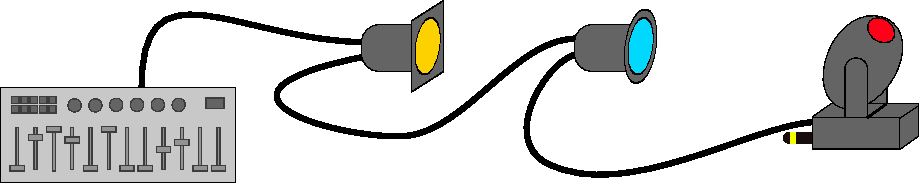
\includegraphics[width=1.00000\textwidth]{Bilder/dmx-line-diagram.pdf}
\caption[Schematical DMX lighting setup example]{Schematical DMX lighting setup example.}\label{fig:dmx-line}
\end{figure}

The DMX signal basically consists of 512 integer values between 0 and
255, each representing the value of one channel. Every fixture \(f\) in
the DMX line listens to a specific number \(n_f\) of these channels
(fixed by the manufacturer) to control its features. The user now has to
give each fixture an address \(a_f\) to mark the first channel it has to
listen to, e.g.~via a DIP switch or a small display on each of the
fixtures. The order of the addresses given to the fixtures does not have
to match the order of the fixtures in the line.

To show how this works in practice, the example is continued (see also
\cref{tbl:dmx-addresses}): At first, the LED head lamp is given address
\(a_{LED} = 1\). It needs \(n_{LED} = 3\) channels to control its red,
green and blue (RGB) components separately, thus listens to channels 1,
2 and 3. To make the LED light yellow, we would need to set channels 1
and 2 (red and green) to 255 and channel 3 (blue) to 0. The next address
we can assign without conflict is \(a_{LED} + n_{LED} = 4\). We give
this address to the dimmer (\(a_{dim} = 4\)) which needs only this one
channel to control its brightness. Now we reserve address 5 for future
use of another dimmer, so that the two dimmer channels will be next to
each other on the desk console. Finally the moving head is assigned
address \(a_{mov} = 6\). We assume that its RGB values, pan / tilt
movement and gobo wheel\footnote{A gobo is a stencil in front of the
  lamp that shapes the emitted light beam. Typically, multiple gobos are
  mounted in a wheel that rotates according to the DMX value in the
  corresponding channel to allow the selection of one gobo at a time.}
can be controlled and therefore 6 channels are needed.

\hypertarget{tbl:dmx-addresses}{}
\begin{longtable}[]{@{}llll@{}}
\caption[Example DMX addresses and channel
numbers]{\label{tbl:dmx-addresses}Example DMX addresses and channel
numbers. }\tabularnewline
\toprule
\begin{minipage}[b]{0.17\columnwidth}\raggedright\strut
fixture\strut
\end{minipage} & \begin{minipage}[b]{0.12\columnwidth}\raggedright\strut
address\strut
\end{minipage} & \begin{minipage}[b]{0.15\columnwidth}\raggedright\strut
number of channels\strut
\end{minipage} & \begin{minipage}[b]{0.28\columnwidth}\raggedright\strut
controlled channels\strut
\end{minipage}\tabularnewline
\midrule
\endfirsthead
\toprule
\begin{minipage}[b]{0.17\columnwidth}\raggedright\strut
fixture\strut
\end{minipage} & \begin{minipage}[b]{0.12\columnwidth}\raggedright\strut
address\strut
\end{minipage} & \begin{minipage}[b]{0.15\columnwidth}\raggedright\strut
number of channels\strut
\end{minipage} & \begin{minipage}[b]{0.28\columnwidth}\raggedright\strut
controlled channels\strut
\end{minipage}\tabularnewline
\midrule
\endhead
\begin{minipage}[t]{0.17\columnwidth}\raggedright\strut
LED head\strut
\end{minipage} & \begin{minipage}[t]{0.12\columnwidth}\raggedright\strut
1\strut
\end{minipage} & \begin{minipage}[t]{0.15\columnwidth}\raggedright\strut
3\strut
\end{minipage} & \begin{minipage}[t]{0.28\columnwidth}\raggedright\strut
ch.~1: red\strut
\end{minipage}\tabularnewline
\begin{minipage}[t]{0.17\columnwidth}\raggedright\strut
\strut
\end{minipage} & \begin{minipage}[t]{0.12\columnwidth}\raggedright\strut
\strut
\end{minipage} & \begin{minipage}[t]{0.15\columnwidth}\raggedright\strut
\strut
\end{minipage} & \begin{minipage}[t]{0.28\columnwidth}\raggedright\strut
ch.~2: green\strut
\end{minipage}\tabularnewline
\begin{minipage}[t]{0.17\columnwidth}\raggedright\strut
\strut
\end{minipage} & \begin{minipage}[t]{0.12\columnwidth}\raggedright\strut
\strut
\end{minipage} & \begin{minipage}[t]{0.15\columnwidth}\raggedright\strut
\strut
\end{minipage} & \begin{minipage}[t]{0.28\columnwidth}\raggedright\strut
ch.~3: blue\strut
\end{minipage}\tabularnewline
\midrule
\begin{minipage}[t]{0.17\columnwidth}\raggedright\strut
dimmer\strut
\end{minipage} & \begin{minipage}[t]{0.12\columnwidth}\raggedright\strut
4\strut
\end{minipage} & \begin{minipage}[t]{0.15\columnwidth}\raggedright\strut
1\strut
\end{minipage} & \begin{minipage}[t]{0.28\columnwidth}\raggedright\strut
ch.~4: brightness\strut
\end{minipage}\tabularnewline
\midrule
\begin{minipage}[t]{0.17\columnwidth}\raggedright\strut
unused\strut
\end{minipage} & \begin{minipage}[t]{0.12\columnwidth}\raggedright\strut
\strut
\end{minipage} & \begin{minipage}[t]{0.15\columnwidth}\raggedright\strut
\strut
\end{minipage} & \begin{minipage}[t]{0.28\columnwidth}\raggedright\strut
ch.~5: --\strut
\end{minipage}\tabularnewline
\midrule
\begin{minipage}[t]{0.17\columnwidth}\raggedright\strut
moving head\strut
\end{minipage} & \begin{minipage}[t]{0.12\columnwidth}\raggedright\strut
6\strut
\end{minipage} & \begin{minipage}[t]{0.15\columnwidth}\raggedright\strut
6\strut
\end{minipage} & \begin{minipage}[t]{0.28\columnwidth}\raggedright\strut
ch.~6: red\strut
\end{minipage}\tabularnewline
\begin{minipage}[t]{0.17\columnwidth}\raggedright\strut
\strut
\end{minipage} & \begin{minipage}[t]{0.12\columnwidth}\raggedright\strut
\strut
\end{minipage} & \begin{minipage}[t]{0.15\columnwidth}\raggedright\strut
\strut
\end{minipage} & \begin{minipage}[t]{0.28\columnwidth}\raggedright\strut
ch.~7: green\strut
\end{minipage}\tabularnewline
\begin{minipage}[t]{0.17\columnwidth}\raggedright\strut
\strut
\end{minipage} & \begin{minipage}[t]{0.12\columnwidth}\raggedright\strut
\strut
\end{minipage} & \begin{minipage}[t]{0.15\columnwidth}\raggedright\strut
\strut
\end{minipage} & \begin{minipage}[t]{0.28\columnwidth}\raggedright\strut
ch.~8: blue\strut
\end{minipage}\tabularnewline
\begin{minipage}[t]{0.17\columnwidth}\raggedright\strut
\strut
\end{minipage} & \begin{minipage}[t]{0.12\columnwidth}\raggedright\strut
\strut
\end{minipage} & \begin{minipage}[t]{0.15\columnwidth}\raggedright\strut
\strut
\end{minipage} & \begin{minipage}[t]{0.28\columnwidth}\raggedright\strut
ch.~9: pan movement\strut
\end{minipage}\tabularnewline
\begin{minipage}[t]{0.17\columnwidth}\raggedright\strut
\strut
\end{minipage} & \begin{minipage}[t]{0.12\columnwidth}\raggedright\strut
\strut
\end{minipage} & \begin{minipage}[t]{0.15\columnwidth}\raggedright\strut
\strut
\end{minipage} & \begin{minipage}[t]{0.28\columnwidth}\raggedright\strut
ch.~10: tilt movement\strut
\end{minipage}\tabularnewline
\begin{minipage}[t]{0.17\columnwidth}\raggedright\strut
\strut
\end{minipage} & \begin{minipage}[t]{0.12\columnwidth}\raggedright\strut
\strut
\end{minipage} & \begin{minipage}[t]{0.15\columnwidth}\raggedright\strut
\strut
\end{minipage} & \begin{minipage}[t]{0.28\columnwidth}\raggedright\strut
ch.~11: gobo wheel\strut
\end{minipage}\tabularnewline
\bottomrule
\end{longtable}

The 512 channels being signalled through one line are called a \emph{DMX
universe}. A desk console can output multiple universes, which allows to
address more fixtures in total.

Instead of using a physical DMX desk, its task can also be fulfilled by
a software. The computer running it is then connected to the DMX line
via a physical interface.

\hypertarget{sec:splitters-mergers}{\subsubsection{DMX Splitters and
Mergers}\label{sec:splitters-mergers}}

There are two notable hardware components that can be used in a DMX line
to make the wiring between fixtures and DMX sources more flexible:

\begin{itemize}
\tightlist
\item
  A DMX splitter is used as a T piece to forward one input signal into
  two (or more) output lines.
\item
  A DMX merger combines the signals from its two input universes
  \emph{A} and \emph{B} (seldomly also more) into one output signal.
  Mergers typically have different modes of operation, such as the
  following. \citep{showtec-dmx-merge}

  \begin{itemize}
  \tightlist
  \item
    \emph{Backup}: As long as \emph{A} is a valid signal, loop it
    through; else use \emph{B}.
  \item
    \emph{Merge}: Use \emph{A}'s first \(x\) channels, then fill the
    remaining 512 minus \(x\) channels with \emph{B}'s first channels.
  \item
    \emph{LTP} (``latest takes precedence''): Loop the universe through
    that has changed later. Sometimes this algorithm is also applied per
    channel instead of per universe.
  \item
    \emph{HTP} (``highest takes precedence''): For each of the 512
    channels, use the highest value of the both corresponding channels
    in \emph{A} and \emph{B}.
  \end{itemize}
\end{itemize}

\hypertarget{sec:dmx-protocol}{\subsection{DMX
protocol}\label{sec:dmx-protocol}}

This section gives a short summary of the official \emph{DMX512-A}
standard \citep{esta-dmx512-a} by the \emph{Entertainment Services and
Technology Association} (\emph{ESTA}).

The DMX protocol defines a serial signal (shown in
\cref{fig:dmx-timing}) at a baud rate of 250000 bits per second. It
consists of individual packets, each of which is initiated by the
\emph{reset sequence} (an arbitrarily long \colorbox{WhiteSmoke}{\lstinline!low!} \emph{BREAK}
signal followed by the \colorbox{WhiteSmoke}{\lstinline!high!} \emph{mark after BREAK}
(\emph{MAB}) and slot 0). A slot contains 8-bit data (least significant
bit first), prepended by a \colorbox{WhiteSmoke}{\lstinline!low!} start bit and followed by two
\colorbox{WhiteSmoke}{\lstinline!high!} stop bits. The data in slot 0 is called the \emph{start
code}, it is always \colorbox{WhiteSmoke}{\lstinline!0x00!} for DMX packets. Other start codes
can be used to indicate manufacturer-specific information or special
functions; those packets shall be ignored by standard DMX receivers, so
they are not relevant in this project.

After the reset sequence, the channel values of the universe are
transmitted in one slot each. Since channels are transmitted serially,
it is possible for fixtures in the DMX line to count received channels
and start listening as soon as their address matches the current channel
number. The channel number therefore does not have to be transmitted
separately. Slots can be separated by a \colorbox{WhiteSmoke}{\lstinline!high!} \emph{mark
between slots} (\emph{MBS}\footnote{This abbreviation is not used in the
  official standard. I introduced it for simpler referencing.}).

Following the last channel, a \colorbox{WhiteSmoke}{\lstinline!high!} \emph{mark before BREAK}
(\emph{MBB}) or the next BREAK indicates the end of the packet. At least
one packet per second should be transmitted, though faster updates are
desirable to ensure fast respondence of the fixtures and, in particular,
smooth light fading. To increase the refresh rate, not all 512 channels
have to be transmitted in a packet.

\begin{figure}
\centering
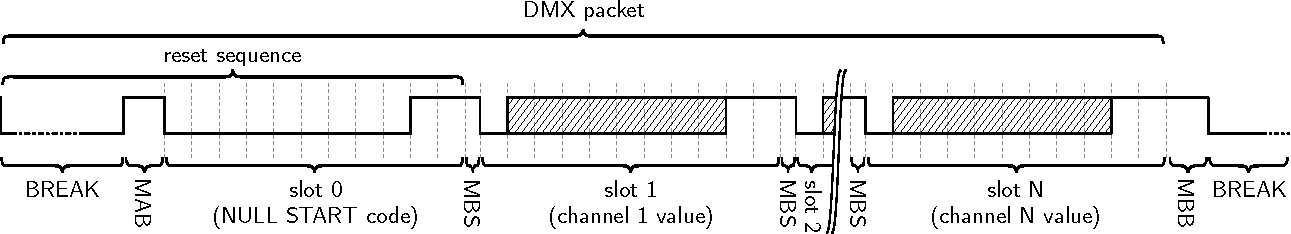
\includegraphics[width=1.00000\textwidth]{Bilder/dmx-timing.pdf}
\caption[DMX timing diagram]{DMX timing diagram.}\label{fig:dmx-timing}
\end{figure}

\hypertarget{tbl:dmx-timing}{}
\begin{longtable}[]{@{}lccc@{}}
\caption[DMX timing]{\label{tbl:dmx-timing}DMX timing. Values in parenthesis only
apply to receivers. From \citep{esta-dmx512-a} }\tabularnewline
\toprule
\begin{minipage}[b]{0.31\columnwidth}\raggedright\strut
Entity\strut
\end{minipage} & \begin{minipage}[b]{0.18\columnwidth}\centering\strut
Min\strut
\end{minipage} & \begin{minipage}[b]{0.18\columnwidth}\centering\strut
Typical\strut
\end{minipage} & \begin{minipage}[b]{0.18\columnwidth}\centering\strut
Max\strut
\end{minipage}\tabularnewline
\midrule
\endfirsthead
\toprule
\begin{minipage}[b]{0.31\columnwidth}\raggedright\strut
Entity\strut
\end{minipage} & \begin{minipage}[b]{0.18\columnwidth}\centering\strut
Min\strut
\end{minipage} & \begin{minipage}[b]{0.18\columnwidth}\centering\strut
Typical\strut
\end{minipage} & \begin{minipage}[b]{0.18\columnwidth}\centering\strut
Max\strut
\end{minipage}\tabularnewline
\midrule
\endhead
\begin{minipage}[t]{0.31\columnwidth}\raggedright\strut
Bit rate\strut
\end{minipage} & \begin{minipage}[t]{0.18\columnwidth}\centering\strut
245kbit/s\strut
\end{minipage} & \begin{minipage}[t]{0.18\columnwidth}\centering\strut
250kbit/s\strut
\end{minipage} & \begin{minipage}[t]{0.18\columnwidth}\centering\strut
255kbit/s\strut
\end{minipage}\tabularnewline
\begin{minipage}[t]{0.31\columnwidth}\raggedright\strut
Bit time\strut
\end{minipage} & \begin{minipage}[t]{0.18\columnwidth}\centering\strut
3.92µs\strut
\end{minipage} & \begin{minipage}[t]{0.18\columnwidth}\centering\strut
4µs\strut
\end{minipage} & \begin{minipage}[t]{0.18\columnwidth}\centering\strut
4.08µs\strut
\end{minipage}\tabularnewline
\midrule
\begin{minipage}[t]{0.31\columnwidth}\raggedright\strut
BREAK\strut
\end{minipage} & \begin{minipage}[t]{0.18\columnwidth}\centering\strut
92µs (88µs)\strut
\end{minipage} & \begin{minipage}[t]{0.18\columnwidth}\centering\strut
176µs\strut
\end{minipage} & \begin{minipage}[t]{0.18\columnwidth}\centering\strut
--\strut
\end{minipage}\tabularnewline
\begin{minipage}[t]{0.31\columnwidth}\raggedright\strut
MAB\strut
\end{minipage} & \begin{minipage}[t]{0.18\columnwidth}\centering\strut
12µs (8µs)\strut
\end{minipage} & \begin{minipage}[t]{0.18\columnwidth}\centering\strut
--\strut
\end{minipage} & \begin{minipage}[t]{0.18\columnwidth}\centering\strut
\textless{} 1.00s\strut
\end{minipage}\tabularnewline
\begin{minipage}[t]{0.31\columnwidth}\raggedright\strut
MBS\strut
\end{minipage} & \begin{minipage}[t]{0.18\columnwidth}\centering\strut
0\strut
\end{minipage} & \begin{minipage}[t]{0.18\columnwidth}\centering\strut
--\strut
\end{minipage} & \begin{minipage}[t]{0.18\columnwidth}\centering\strut
\textless{} 1.00s\strut
\end{minipage}\tabularnewline
\begin{minipage}[t]{0.31\columnwidth}\raggedright\strut
MBB\strut
\end{minipage} & \begin{minipage}[t]{0.18\columnwidth}\centering\strut
0\strut
\end{minipage} & \begin{minipage}[t]{0.18\columnwidth}\centering\strut
--\strut
\end{minipage} & \begin{minipage}[t]{0.18\columnwidth}\centering\strut
\textless{} 1.00s\strut
\end{minipage}\tabularnewline
\begin{minipage}[t]{0.31\columnwidth}\raggedright\strut
DMX packet\strut
\end{minipage} & \begin{minipage}[t]{0.18\columnwidth}\centering\strut
1204µs (1196µs)\strut
\end{minipage} & \begin{minipage}[t]{0.18\columnwidth}\centering\strut
--\strut
\end{minipage} & \begin{minipage}[t]{0.18\columnwidth}\centering\strut
1.00s (1.25s)\strut
\end{minipage}\tabularnewline
\begin{minipage}[t]{0.31\columnwidth}\raggedright\strut
Refresh rate\strut
\end{minipage} & \begin{minipage}[t]{0.18\columnwidth}\centering\strut
830Hz (836Hz)\strut
\end{minipage} & \begin{minipage}[t]{0.18\columnwidth}\centering\strut
--\strut
\end{minipage} & \begin{minipage}[t]{0.18\columnwidth}\centering\strut
1Hz (0.8Hz)\strut
\end{minipage}\tabularnewline
\bottomrule
\end{longtable}

If one considers packets with all 512 channels, one can work out from
\cref{tbl:dmx-timing} a minimum packet time of 22.7ms, or a maximum
refresh rate of 44Hz.

An extension to DMX that will not be important for this thesis but
should still be mentioned is \emph{Remote Device Management}
(\emph{RDM}). It allows setting the fixtures' DMX address and other
options from the RDM controller, which is an extended DMX desk or
software. It works by interleaving the unidirectional DMX signal with
bidirectional RDM packets.

\hypertarget{sec:dmx-electrical}{\subsubsection{Electrical
specification}\label{sec:dmx-electrical}}

DMX uses the electrical specifications defined in the industry standard
EIA-485 (also known as RS-485) which describes balanced
transmission-line signaling \citep{texas-instruments-eia-485}.
``Balanced'' means data bits are encoded via the potential difference
between the twisted-pair cables \emph{Data~+} and \emph{Data~--}. This
decreases interference liability, since noise adds to both data lines
equally -- effectively cancelling itself out in the difference --, and
thus makes line lengths of up to 1.2km possible. For DMX lines though,
the recommendation is to stay below 300m \citep{bennette-practice}.

\begin{figure}
\centering
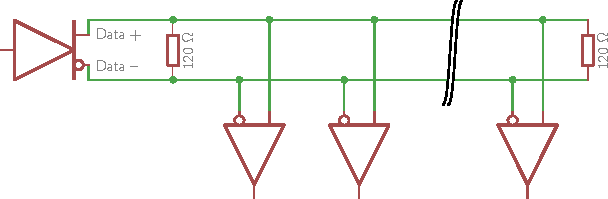
\includegraphics[width=0.90000\textwidth]{Bilder/eia-485-bus.pdf}
\caption[EIA-485 bus with one transmitter and up to 32
receivers]{EIA-485 bus with one transmitter and up to 32
receivers.}\label{fig:eia-485-bus}
\end{figure}

In \cref{fig:eia-485-bus}, the electrical schematic of such a bus is
shown. On the left, the transmitter converts the raw signal into the
differential signal. All the receivers on the bottom (up to 32 are
allowed) do the same in the other direction.\footnote{Actually, all
  devices connected to the bus are allowed to both transmit and receive
  (e.g.~used in RDM). Thus, usually so-called ``bus transceiver chips''
  that can convert in both directions are deployed. Since communication
  over DMX will always be uni-directional in this thesis, I simplified
  the figure.} At both the near end (transmitter side) and the far end
(after last receiver), a termination resistor of 120 ohms is installed
to minimize reflections that could interfere with the signal.

The DMX standard requires 5-pin XLR connectors, except where they are
``physically impossible to mount'' \citep{esta-dmx512-a}. Even so, most
DMX hardware is equipped with a 3-pin XLR connector instead or
additionally. This is due to the fact that only 3 pins are needed and
3-pin XLR cables are common in event technology because they are also
used for microphones.

\begin{figure}
\centering
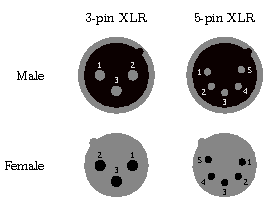
\includegraphics[width=0.50000\textwidth]{Bilder/xlr-connectors.pdf}
\caption[XLR connectors used for DMX]{XLR connectors used for DMX.}\label{fig:xlr-connectors}
\end{figure}

\hypertarget{tbl:xlr-pins}{}
\begin{longtable}[]{@{}ccc@{}}
\caption[XLR pin assignment for DMX]{\label{tbl:xlr-pins}XLR pin assignment for DMX.
}\tabularnewline
\toprule
Pin Number & 3-pin XLR & 5-pin XLR\tabularnewline
\midrule
\endfirsthead
\toprule
Pin Number & 3-pin XLR & 5-pin XLR\tabularnewline
\midrule
\endhead
1 & Ground & Ground\tabularnewline
2 & \emph{Data --} & \emph{Data --}\tabularnewline
3 & \emph{Data +} & \emph{Data +}\tabularnewline
4 & -- & \emph{Data 2 --} (optional)\tabularnewline
5 & -- & \emph{Data 2 +} (optional)\tabularnewline
\bottomrule
\end{longtable}

\hypertarget{sec:art-net-sacn}{\subsection{Art-Net and sACN
protocols}\label{sec:art-net-sacn}}

DMX only allows one or two universes per line, which may make cabling
impractical in some use cases. To overcome this issue, the English
lighting equipment company \emph{Artistic Licence} created a free-to-use
DMX over UDP\footnote{User Datagram Protocol} protocol called
\emph{Art-Net} \citep{artistic-licence-art-net4} in 1998. It allows
sending multiple DMX universes over a standard IP network and thus
highly extends the flexibility of lighting systems since a single
Ethernet link or a wireless network can be used for large parts of the
transport way.

There are lighting controllers and fixtures that work directly with
Art-Net (exclusively or alongside traditional DMX), all others can be
connected via an \emph{Art-Net Node} that converts to and from DMX.
Often, the protocol is used for communication between a lighting
software on a computer and one such Node acting as the DMX source for
fixtures, like in \cref{fig:art-net-node-schematic}.

\begin{figure}
\centering
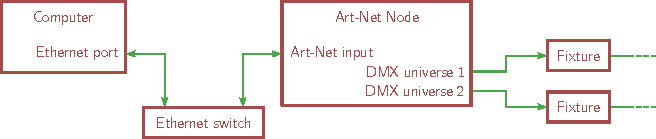
\includegraphics[width=1.00000\textwidth]{Bilder/art-net-node-schematic.pdf}
\caption[Schematical connection of an Art-Net
Node]{Schematical connection of an Art-Net
Node.}\label{fig:art-net-node-schematic}
\end{figure}

\emph{Streaming ACN} (\emph{sACN}), which was standardized as ANSI E1.31
in late 2016 \citep{esta-sacn}, is ESTA's open protocol with the same
goals and shares most of its high level properties with Art-Net. In this
thesis, the details and differences of both protocols will not be
covered.

\hypertarget{sec:uart}{\section{UART}\label{sec:uart}}

The \emph{Universal Asynchronous Receiver Transmitter} (\emph{UART}) is
an interface present on many microcontrollers that allows communication
over serial bus lines. There is no extra clock signal, the receiver
synchronizes itself through the fixed data format: Data bits are
transmitted sequentially, framed in slots with \colorbox{WhiteSmoke}{\lstinline!low!} start and
\colorbox{WhiteSmoke}{\lstinline!high!} stop bits. If the signal is \colorbox{WhiteSmoke}{\lstinline!low!} for longer
than one slot time, the \emph{break condition} is fulfilled.

Various parameters have to be fixed at both receiver and transmitter to
avoid misunderstanding: Baud rate, the number of data bits per slot
(usually 5 to 9), bit numbering (most or least significant bit first),
the number of stop bits used (one or two) and if each slot should
additionally contain a parity bit.

As the \protect\hyperlink{sec:dmx-protocol}{DMX timing protocol} is a
specialization of this specification, sending and receiving DMX data via
a UART is possible. One caveat though is the non-standard baud rate of
250kbit/s.

\hypertarget{sec:spi}{\section{SPI}\label{sec:spi}}

The \emph{Serial Peripheral Interface} (\emph{SPI}) is a synchronous
data transmission interface between a master and multiple slave devices
designed by Motorola \citep{dembowski-raspi}. Only the independent slave
configuration will be discussed here, which can be seen in
\cref{fig:spi-schematic}.

\begin{figure}
\centering
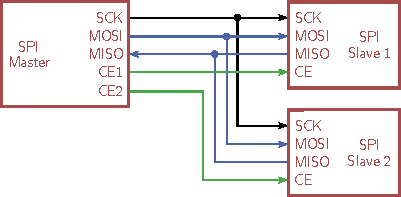
\includegraphics[width=0.60000\textwidth]{Bilder/spi-schematic.pdf}
\caption[Schematic of SPI master and slaves]{Schematic of SPI master and slaves.}\label{fig:spi-schematic}
\end{figure}

By applying a \colorbox{WhiteSmoke}{\lstinline!low!} signal at one of the \emph{Slave select} /
\emph{Chip enable} (\emph{CE}) pins, the master can notify the
corresponding slave that it wants to communicate with. After that, the
master generates a clock signal at the \emph{SCK} (\emph{Serial clock})
pin and simultaneously reads at the \emph{MISO} (\emph{Master In, Slave
Out}) pin and transmits at the \emph{MOSI} (\emph{Master Out, Slave In})
pin one bit per clock cycle. After the data transmission is completed
(e.g.~one byte is sent to the slave who then may answer with one byte,
but that depends on the protocol fixed between the devices), the master
resets all pins to their idle levels.

There are multiple SPI modes that define when the bit read / write
operation should happen in relation to the clock signal. For simplicity,
only mode 0 is shown here, in which \emph{SCK}'s idle status is
\colorbox{WhiteSmoke}{\lstinline!low!} and data transfer starts with the first rising edge in
the clock signal (see \cref{fig:spi-timing}).

\begin{figure}
\centering
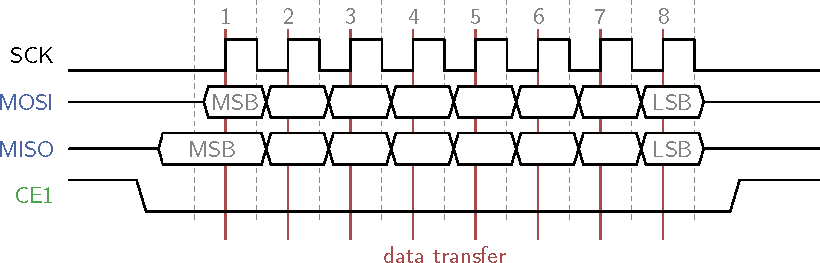
\includegraphics[width=0.90000\textwidth]{Bilder/spi-timing.pdf}
\caption[SPI timing diagram]{SPI timing diagram. MSB and LSB are short for \emph{most
significant bit} and \emph{least significant bit}, respectively. Adapted
from \citep{dembowski-raspi}.}\label{fig:spi-timing}
\end{figure}

\cleardoublepage\hypertarget{sec:system-design}{\chapter{Requirement analysis and system
design}\label{sec:system-design}}

In this chapter, the plan for the PC-DMX interface is outlined. First, I
will define my \protect\hyperlink{sec:requirements}{requirements} and
examine several existing \protect\hyperlink{sec:market-study}{products
on the market} on how they match or fail these requirements. This will
then lead to the \protect\hyperlink{sec:design}{design} of the interface
described in this thesis.

\hypertarget{sec:requirements}{\section{Requirement
analysis}\label{sec:requirements}}

The requirements defined in this section are designed for the specific
use case of small associations like technics teams in youth groups
(i.e.~not professional event management companies or the like). Their
budget is usually very limited but their expertise does not have to be
-- i.e.~the PC-DMX interface must offer features for advanced users
while still being affordable.

A youth technics team may not have found its optimum workflow yet and
may want to improve it by trying out different free lighting control
programs, e.g.~QLC+\footnote{\url{http://www.qlcplus.org/}}, DMX
Control\footnote{\url{https://www.dmxcontrol.org/}} or FreeStyler
DMX\footnote{\url{http://www.freestylerdmx.be/}}. The interface should
support that by being compatible with as many of them as possible.

Connection to the computer shall be possible via Ethernet to allow
extending the cable via standard network equipment like switches,
routers and Wi-Fi access points. USB connection is not sufficient
because USB devices need special drivers and configuration, which would
make the interface less portable, e.g.~if a quick replacement computer
in an emergency situation is needed. Among the protocols used for data
transmission, at least one should be open, i.e.~either sACN or
Art-Net\footnote{Although Art-Net is not strictly open, it is
  free-to-use and supported by a wide variety of software and hardware.}
should be supported.

The interface should support output of at least two DMX universes to be
able to address a sufficiently large number of fixtures and input of at
least one to allow haptic control of DMX channels using a mixing desk.
The method how DMX input signals are handled should be configurable:

\begin{itemize}
\tightlist
\item
  Either the DMX channel values are sent via Art-Net to the control
  software (default \emph{Art-Net Node}-like mode), e.g.~to control
  software functions with hardware mixing desk faders,
\item
  or it acts like a \protect\hyperlink{sec:splitters-mergers}{DMX
  splitter}, forwarding its DMX input signal on both DMX outputs,
\item
  or the DMX input channels are merged with the channel values provided
  over the network into one of the output universes using one of the
  merge modes described in \cref{sec:splitters-mergers}.
\end{itemize}

All input and output DMX signals should be processed with a high refresh
frequency, so that delays remain low and smooth light fading is
possible.

Using the interface should be as simple as possible for end-users. That
means that neither in-depth knowledge about the DMX protocol or computer
networks nor special know-how about this specific interface should be
required to use it. However, end-users are assumed to know how to work
with DMX software and hardware in general. More complicated functions
like the flexible input mapping mentioned above should be trivial enough
to be understandable in a short period of time.

The whole setup should cost less than 100\euro{} and be extensible,
i.e.~widened future requirements like the need for more DMX universes
should be easy to implement without a redesign and rebuild of the whole
hardware and software.

Additionally, it would be appreciated if both hardware and software were
open-source to allow others to extend and improve the interface.

\hypertarget{sec:market-study}{\section{Market
study}\label{sec:market-study}}

A market study was conducted to see how existing products do fulfill the
requirements defined in the previous section. The price limit on
100\euro{} was fixed to narrow down the products in the first step. An
overview of the products described here is given in
\cref{tbl:market-overview}.

Since the price limit of 100\euro{} narrows down the range of
professional hardware to various USB-to-DMX adapters and one Art-Net
Node by \emph{Eurolite}\footnote{\url{https://www.steinigke.de/en/mpn70064842-eurolite-art-net-dmx-node-1.html}}
-- all of them with support for only one output universe, none with DMX
input --, only ``Do It Yourself'' projects are left.

A popular one, \emph{DMXControl Projects}' \emph{Nodle U1}\footnote{\url{https://www.dmxcontrol-projects.org/hardware/nodle-u1.html}},
can also only be connected via USB. Thus, it has to be explicitly
supported by lighting programs -- which several do. Nevertheless, it
fails the network connection requirement.

Some members of the \emph{DMXControl} forum and wiki created an Art-Net
Node based on a commercially available AVR construction kit\footnote{\url{https://wiki.dmxcontrol.de/wiki/Art-Net-Node_f\%C3\%BCr_25_Euro}}.
It was refined and eventually ported to its own hardware to support two
DMX universes\footnote{\url{https://wiki.dmxcontrol.de/wiki/ArtNetNode_auf_einer_Platine}}.
Unfortunately, this is still not sufficient.

The same applies to GitHub user \emph{mtongnz}'s Art-Net Node based on
the Wi-Fi-enabled \emph{ESP8266} microcontroller\footnote{\url{https://github.com/mtongnz/ESP8266_ArtNetNode_v2}}.

The project that matches most of my requirements is the \emph{Quad Art
Net Box} by Ulrich Radig\footnote{\url{https://www.ulrichradig.de/home/index.php/dmx/quad-art-net}}:
It supports four DMX output universes, one of them can be toggled to an
input. Sources and schematics are available online, and an assembly kit
can be ordered. However, there is no information given about whether the
DMX input can be flexibly merged into one DMX output universe or if it
is always forwarded to the Art-Net output.

Rather than doing all the work in one microcontroller like in the
previous projects, \emph{raspberrypi-dmx.org}\footnote{\url{http://www.raspberrypi-dmx.org/raspberry-pi-art-net-dmx-out}}
uses a much more powerful Raspberry Pi with an additional co-processor
on an extension board (sometimes called \emph{shield}) that is plugged
into the GPIO (General Purpose Input / Output) pins. Thereby, only the
software needs to be replaced (by re-flashing the SD card) to match the
use case: USB, Art-Net, sACN, Open Sound Control and MIDI can all be
converted to DMX with the correct SD card image. Unfortunately, the
extension board hardware does only support one input and one output
universe.

\hypertarget{tbl:market-overview}{}
{
\renewcommand{\arraystretch}{2}
\begin{longtable}[]{@{}lcccc@{}}
\caption[Available products
overview]{\label{tbl:market-overview}Available products
overview. Values in parenthesis specify alternate modes.
}\tabularnewline
\toprule
\begin{minipage}[b]{0.29\columnwidth}\raggedright\strut
Product\strut
\end{minipage} & \begin{minipage}[b]{0.18\columnwidth}\centering\strut
Simultaneous output / input universes\strut
\end{minipage} & \begin{minipage}[b]{0.11\columnwidth}\centering\strut
Flexible input mapping\strut
\end{minipage} & \begin{minipage}[b]{0.14\columnwidth}\centering\strut
Open / Extensible\strut
\end{minipage} & \begin{minipage}[b]{0.14\columnwidth}\centering\strut
Connection to computer\strut
\end{minipage}\tabularnewline
\midrule
\endfirsthead
\toprule
\begin{minipage}[b]{0.29\columnwidth}\raggedright\strut
Product\strut
\end{minipage} & \begin{minipage}[b]{0.18\columnwidth}\centering\strut
Simultaneous output / input universes\strut
\end{minipage} & \begin{minipage}[b]{0.11\columnwidth}\centering\strut
Flexible input mapping\strut
\end{minipage} & \begin{minipage}[b]{0.14\columnwidth}\centering\strut
Open / Extensible\strut
\end{minipage} & \begin{minipage}[b]{0.14\columnwidth}\centering\strut
Connection to computer\strut
\end{minipage}\tabularnewline
\midrule
\endhead
\begin{minipage}[t]{0.29\columnwidth}\raggedright\strut
Professional USB-to-DMX~adapters\strut
\end{minipage} & \begin{minipage}[t]{0.18\columnwidth}\centering\strut
1 \textcolor{FireBrick}{\ding{55}} / 0
\textcolor{FireBrick}{\ding{55}}\strut
\end{minipage} & \begin{minipage}[t]{0.11\columnwidth}\centering\strut
\emph{N/A} \textcolor{FireBrick}{\ding{55}}\strut
\end{minipage} & \begin{minipage}[t]{0.14\columnwidth}\centering\strut
\textcolor{FireBrick}{\ding{55}} /
\textcolor{FireBrick}{\ding{55}}\strut
\end{minipage} & \begin{minipage}[t]{0.14\columnwidth}\centering\strut
USB \textcolor{FireBrick}{\ding{55}}\strut
\end{minipage}\tabularnewline
\begin{minipage}[t]{0.29\columnwidth}\raggedright\strut
Eurolite Art-Net/DMX~Node~1\strut
\end{minipage} & \begin{minipage}[t]{0.18\columnwidth}\centering\strut
1 \textcolor{FireBrick}{\ding{55}} / 0
\textcolor{FireBrick}{\ding{55}}\strut
\end{minipage} & \begin{minipage}[t]{0.11\columnwidth}\centering\strut
\emph{N/A} \textcolor{FireBrick}{\ding{55}}\strut
\end{minipage} & \begin{minipage}[t]{0.14\columnwidth}\centering\strut
\textcolor{FireBrick}{\ding{55}} /
\textcolor{FireBrick}{\ding{55}}\strut
\end{minipage} & \begin{minipage}[t]{0.14\columnwidth}\centering\strut
Art-Net \textcolor{ForestGreen}{\ding{51}}\strut
\end{minipage}\tabularnewline
\begin{minipage}[t]{0.29\columnwidth}\raggedright\strut
DMXControl~Projects Nodle~U1\strut
\end{minipage} & \begin{minipage}[t]{0.18\columnwidth}\centering\strut
1 \textcolor{FireBrick}{\ding{55}} / 1
\textcolor{ForestGreen}{\ding{51}}\strut
\end{minipage} & \begin{minipage}[t]{0.11\columnwidth}\centering\strut
\textcolor{FireBrick}{\ding{55}}\strut
\end{minipage} & \begin{minipage}[t]{0.14\columnwidth}\centering\strut
\textcolor{ForestGreen}{\ding{51}} / \textcolor{FireBrick}{\ding{55}}
\footnotemark{}\strut
\end{minipage}
\footnotetext{\emph{DMXControl Projects} do state in their manual that
  ``future extensions should be possible''\citep{dmxcontrol-nodle-u1}.
  However it seems to me that such extensions would still require
  completely redesigned hardware.} &
\begin{minipage}[t]{0.14\columnwidth}\centering\strut
USB \textcolor{FireBrick}{\ding{55}}\strut
\end{minipage}\tabularnewline
\begin{minipage}[t]{0.29\columnwidth}\raggedright\strut
DMXControl~Wiki AvrArtNodeV2.0\strut
\end{minipage} & \begin{minipage}[t]{0.18\columnwidth}\centering\strut
2 \textcolor{ForestGreen}{\ding{51}} / 0
\textcolor{FireBrick}{\ding{55}}\\
 (0 \textcolor{FireBrick}{\ding{55}} / 2
\textcolor{ForestGreen}{\ding{51}})\strut
\end{minipage} & \begin{minipage}[t]{0.11\columnwidth}\centering\strut
\emph{N/A} \textcolor{FireBrick}{\ding{55}}\strut
\end{minipage} & \begin{minipage}[t]{0.14\columnwidth}\centering\strut
\textcolor{ForestGreen}{\ding{51}} /
\textcolor{FireBrick}{\ding{55}}\strut
\end{minipage} & \begin{minipage}[t]{0.14\columnwidth}\centering\strut
Art-Net \textcolor{ForestGreen}{\ding{51}}\strut
\end{minipage}\tabularnewline
\begin{minipage}[t]{0.29\columnwidth}\raggedright\strut
mtongnz ESP8266\_ArtNetNode\_v2\strut
\end{minipage} & \begin{minipage}[t]{0.18\columnwidth}\centering\strut
2 \textcolor{ForestGreen}{\ding{51}} / 0
\textcolor{FireBrick}{\ding{55}}\\
 (1 \textcolor{FireBrick}{\ding{55}} / 1
\textcolor{ForestGreen}{\ding{51}})\strut
\end{minipage} & \begin{minipage}[t]{0.11\columnwidth}\centering\strut
\textcolor{FireBrick}{\ding{55}}\strut
\end{minipage} & \begin{minipage}[t]{0.14\columnwidth}\centering\strut
\textcolor{ForestGreen}{\ding{51}} /
\textcolor{FireBrick}{\ding{55}}\strut
\end{minipage} & \begin{minipage}[t]{0.14\columnwidth}\centering\strut
Art-Net \textcolor{ForestGreen}{\ding{51}}\strut
\end{minipage}\tabularnewline
\begin{minipage}[t]{0.29\columnwidth}\raggedright\strut
Ulrich~Radig Quad~Art~Net~Box\strut
\end{minipage} & \begin{minipage}[t]{0.18\columnwidth}\centering\strut
3 \textcolor{ForestGreen}{\ding{51}} / 1
\textcolor{ForestGreen}{\ding{51}}\\
 (4 \textcolor{ForestGreen}{\ding{51}} / 0
\textcolor{FireBrick}{\ding{55}})\strut
\end{minipage} & \begin{minipage}[t]{0.11\columnwidth}\centering\strut
\textcolor{FireBrick}{\ding{55}}\strut
\end{minipage} & \begin{minipage}[t]{0.14\columnwidth}\centering\strut
\textcolor{ForestGreen}{\ding{51}} /
\textcolor{FireBrick}{\ding{55}}\strut
\end{minipage} & \begin{minipage}[t]{0.14\columnwidth}\centering\strut
Art-Net \textcolor{ForestGreen}{\ding{51}}\strut
\end{minipage}\tabularnewline
\begin{minipage}[t]{0.29\columnwidth}\raggedright\strut
Raspberry Pi\\
 Art-Net 3 -\textgreater{} DMX Out\strut
\end{minipage} & \begin{minipage}[t]{0.18\columnwidth}\centering\strut
1 \textcolor{FireBrick}{\ding{55}} / 1
\textcolor{ForestGreen}{\ding{51}}\strut
\end{minipage} & \begin{minipage}[t]{0.11\columnwidth}\centering\strut
\textcolor{FireBrick}{\ding{55}}\strut
\end{minipage} & \begin{minipage}[t]{0.14\columnwidth}\centering\strut
\textcolor{ForestGreen}{\ding{51}} /
\textcolor{ForestGreen}{\ding{51}}\strut
\end{minipage} & \begin{minipage}[t]{0.14\columnwidth}\centering\strut
Art-Net \\
 + others \textcolor{ForestGreen}{\ding{51}}\strut
\end{minipage}\tabularnewline
\bottomrule
\end{longtable}}

Another interesting project I have found during my research is the
\emph{Open Lighting Architecture} (\emph{OLA}) software, which will be
further explained in \cref{sec:ola}. It aims to be a universal protocol
translator for DMX signals, supporting different devices through
plugins. It can be installed on the Raspberry Pi and a plugin providing
native DMX output through its \protect\hyperlink{sec:uart}{UART port} is
already available.

In conclusion, none of the existing products fulfills all requirements,
but there are a few different approaches and projects that provide a
good starting point for building an PC-DMX interface myself.

\hypertarget{sec:design}{\section{System design}\label{sec:design}}

The single-board computer Raspberry Pi will form the basis of the
adapter. It has Ethernet and USB ports and a CPU powerful enough to run
OLA. An extension board interfaced to its GPIO pins must be developed.
It has to be equipped with two EIA-485 bus transceivers to provide one
DMX input and, through the aforementioned UART plugin, one output. The
second output will be supplied by an USB-to-DMX adapter that was
available to me, the \emph{DMXCreator 512 Basic}\footnote{\url{http://www.dmx512.ch/512.html}}.
Its protocol has to be reverse-engineered and incorporated into OLA's
USB plugin (see \cref{sec:ola-dmxcreator-plugin}). Initial observation
of the protocol suggested the feasibility of this approach.

An OLA plugin that allows direct DMX input on the Raspberry Pi is yet to
be developed. Initially, I planned to extend the UART plugin. However,
prototyping the protocol recognition using the UART port did not
succeed, so the SPI bus will be used to sample the DMX signal instead.
Further details of this technique are explained in
\cref{sec:ola-spidmx-plugin}.

\begin{figure}
\centering
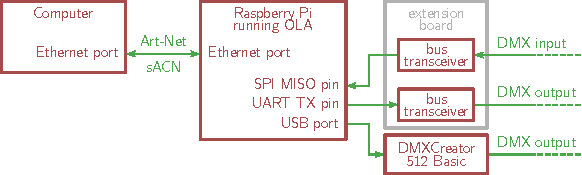
\includegraphics[width=1.00000\textwidth]{Bilder/system-design-schematic.pdf}
\caption[Schematic of the planned PC-DMX
interface]{Schematic of the planned PC-DMX
interface.}\label{fig:system-design-schematic}
\end{figure}

\cleardoublepage\hypertarget{sec:implementation}{\chapter{Implementation}\label{sec:implementation}}

In \cref{sec:system-design}, requirements were specified which the
desired PC-DMX interface has to fulfill. A market study revealed that no
existing products match these requirements, so a system design was
developed. This chapter describes the steps I took to implement this
design.

First, relevant parts of the \emph{Open Lighting Architecture}
(\emph{OLA}) project, which will be used as the software basis, are
outlined, before it is initially installed on a Raspberry Pi.
Afterwards, the physical extension board and implementation of both
required extensions to the OLA software are explained. The build of a
chassis completes this chapter.

\section{The Open Lighting Architecture Project}\label{sec:ola}

The \emph{Open Lighting Architecture} (\emph{OLA}) project I discovered
during my \protect\hyperlink{sec:market-study}{market study} is
described in \citep{lsa-dmx-tester} as

\begin{quote}
{[}\ldots{}{]} free, open source software originally created by Simon
Newton and now developed by a team of contributors around the world. It
runs on Linux or Mac and is capable of interfacing with USB DMX512
hardware, DMX512 over IP protocols, and the Raspberry Pi's GPIO pins.
The application includes a web interface for easily creating,
monitoring, and configuring DMX universes. OLA is one part of the larger
Open Lighting Project, which aims to build high-quality, free software
for the entertainment lighting industry.
\end{quote}

As it provides the basis of my implementation, I briefly explain some
concepts in the project that are needed later.

\subsection{Terminology}\label{terminology}

In OLA, some keywords are used extensively \citep{using-ola}:

\begin{itemize}
\tightlist
\item
  A \emph{port} is a point where at most 512 DMX channel values are
  passed to (\emph{output port}) or read in (\emph{input port}). It can
  either be physical or virtual (like in Art-Net).
\item
  A \emph{device} groups ports together, it consists of at least one
  port.
\item
  A \emph{plugin} provides support for recognizing, connecting to and
  communicating with one or more devices. It has to be compiled along
  with OLA (i.e.~cannot be downloaded and connected afterwards) and thus
  has to be part of the project. At runtime, plugins can be enabled and
  disabled independently.
\item
  An OLA \emph{universe} is an internal set of 512 DMX channel values.
  It can be \emph{patched} by the user to input ports to receive new
  data and / or to output ports to transmit its current channel values.
\end{itemize}

\subsection{Relevant existing plugins}\label{relevant-existing-plugins}

At the time of writing, there are already more than 20 plugins available
in OLA's source code. Amongst them, the following are of special
interest for this thesis.

\subsubsection{Art-Net Plugin}\label{art-net-plugin}

The \emph{ArtNet Plugin}\footnote{\url{https://github.com/OpenLightingProject/ola/tree/master/plugins/artnet}.
  It is actually not named \emph{Art-Net Plugin} at the time of writing.
  I opened issue
  \href{https://github.com/OpenLightingProject/ola/issues/1328}{\#1328}
  on GitHub to fix this.} implements the
\protect\hyperlink{sec:art-net-sacn}{Art-Net protocol} version 3, which
supports at most four input universes and four output universes per IP
address. This plugin creates input ports and output ports accordingly,
which can be patched to OLA universes and thereby relay DMX data to /
from external lighting programs. Since the Art-Net protocol is designed
in a backwards-compatible manner, both newer and older client software
are able to communicate with OLA.

This plugin does not need additional hardware, it uses the network ports
that are already available.

\subsubsection{UART Plugin}\label{sec:ola-uart-plugin}

The \emph{Native UART DMX Plugin}\footnote{\url{https://github.com/OpenLightingProject/ola/tree/master/plugins/uartdmx}}
instantiates one output port that directly generates the
\protect\hyperlink{sec:dmx-protocol}{DMX signal} via the
\protect\hyperlink{sec:uart}{UART port} of the host device, usually a
Raspberry Pi.

This signal at a GPIO pin must then only be run through a bus
transceiver chip to transform it into a balanced EIA-485 signal with a
valid potential difference.

Richard Ash, the initial author of this plugin, outlines the
difficulties he had to face for his implementation in a blog
post\footnote{\url{http://eastertrail.blogspot.de/2014/04/command-and-control-ii.html}}:

\begin{itemize}
\tightlist
\item
  ``DMX-512 runs a a {[}sic{]} non-standard (for PC) baud rate of
  250kbaud.''\\
  Fortunately, this issue could be solved on Linux by using the
  \colorbox{WhiteSmoke}{\lstinline!termios2!} interface for UART setup.
\item
  ``DMX-512 uses serial break signals {[}\ldots{}{]}. These cannot be
  sent by just writing characters out of the serial port.''\\
  Again, the \colorbox{WhiteSmoke}{\lstinline!termios2!} interface provides methods to start
  and end the BREAK. In between, a standard \colorbox{WhiteSmoke}{\lstinline!usleep!} call
  interrupts the sending thread for the specified time; imprecisions do
  not matter in this case.
\item
  ``DMX-512 has relative tight timing requirements for various elements
  of the signal -- if your computer suddenly stops sending data for a
  while, then the lights you are controlling may go out or flicker
  randomly.''\\
  This is true indeed, however both his own project experience and my
  testing have proven the output to be reliable enough for smooth light
  fading.
\end{itemize}

\hypertarget{sec:ola-usb-plugin}{\subsubsection{USB
Plugin}\label{sec:ola-usb-plugin}}

The \emph{USB DMX Plugin}\footnote{\url{https://github.com/OpenLightingProject/ola/tree/master/plugins/usbdmx}}
provides support for a variety of USB-to-DMX adapters. Each of them is
controlled by a ``sub-plugin'' that extends the common basis
implementation. This simplifies access to the \colorbox{WhiteSmoke}{\lstinline!libusb!} library
and reduces code duplication.

Each sub-plugin gets notified about a newly plugged in USB device and
can claim it if vendor ID, device ID and possibly other information
match predefined values. Then, it is responsible for creating ports and
communicating with the device.

\subsubsection{SPI Plugin}\label{sec:ola-spi-plugin}

The \emph{SPI Plugin}\footnote{\url{https://github.com/OpenLightingProject/ola/tree/master/plugins/spi}}
allows to directly operate LED pixel strips with
\protect\hyperlink{sec:spi}{SPI}-controllable LED drivers like WS2801 or
LPD8806\footnote{see \url{https://opendmx.net/index.php/OLA_LED_Pixels}}.
Advanced functions like using hardware SPI multiplexers and multiple
pixel strips are available but beyond the scope of this explanation.

\subsection{Project organization with
GitHub}\label{project-organization-with-github}

The project repository is hosted at GitHub\footnote{\url{https://github.com/OpenLightingProject/ola}}.
Its \colorbox{WhiteSmoke}{\lstinline!master!} branch always contains the newest development
version, released versions are tagged commits in the git history (like
\colorbox{WhiteSmoke}{\lstinline!0.10.5!}). For every bigger version change (like from
\colorbox{WhiteSmoke}{\lstinline!0.9.x!} to \colorbox{WhiteSmoke}{\lstinline!0.10.0!}), a version branch is created
(\colorbox{WhiteSmoke}{\lstinline!0.10!}) that allows future bug fix commits to be targeted
against the released version without having to include newer features
from the \colorbox{WhiteSmoke}{\lstinline!master!} branch.

Pull requests from contributors' forks are automatically run against the
project's tests and linters and have to be approved by both main
developers, Simon Newton and Peter Newman. This allows spotting bugs and
inconsistencies early and ensures good code quality.

\section{Initial setup of OLA on the Raspberry
Pi}\label{initial-setup-of-ola-on-the-raspberry-pi}

In this section, I explain the steps which were needed to install OLA on
a Raspberry Pi 1 model B+ from scratch. Newer versions of the
single-board computer should work as well, but may need some slight
adjustments.

First, a recent Raspbian Lite image from the Raspberry Pi
homepage\footnote{\url{https://raspberrypi.org/downloads/raspbian/}.
  There are also pre-configured OLA images available from
  \url{http://dl.openlighting.org/}, but since I need the latest
  \emph{git} version to apply my own changes and those images were not
  updated for several years, the manual procedure is the better way.}
has to be downloaded and flashed\footnote{Instructions:
  \url{https://raspberrypi.org/documentation/installation/installing-images/README.md}}
onto the microSD card that the Raspberry Pi will boot from. The microSD
card should be at least 4GB in size\footnote{I managed to install OLA on
  a 2GB card, but that required removing various packages and constantly
  scratching at the space limit. I later switched to a 4GB card.}.
Secure shell (SSH) access is disabled by default in Raspbian. Since SSH
is required for connecting remotely to the Raspberry Pi, it must be
enabled by putting a new (empty) file named \colorbox{WhiteSmoke}{\lstinline!ssh!} in the
card's root directory.

After booting up the Raspberry Pi with the newly flashed microSD card
and connecting it to the network with an Ethernet cable, the IP address
has to be found out\footnote{Instructions:
  \url{https://raspberrypi.org/documentation/remote-access/ip-address.md}}
so that a secure shell can be opened. In this shell, all following
commands are executed.

Before continuing, all packages, firmware and the kernel should be
updated to their latest versions:

\begin{lstlisting}[style=myBash]
sudo apt update
sudo apt upgrade
sudo rpi-update
\end{lstlisting}

\subsection{Building and installing
OLA}\label{building-and-installing-ola}

Building OLA from source for the first time takes several hours. Thus,
it may be helpful to overclock Raspberry Pi's processor via
\colorbox{WhiteSmoke}{\lstinline!raspi-config!}; the \emph{Medium} setting worked reliably for
me. A reboot is needed for the change to take effect.

Some prerequisite packages are required for building OLA and need to be
installed with \colorbox{WhiteSmoke}{\lstinline!apt!}. Thereafter, the latest source code from
GitHub is downloaded, built and the resulting binaries get copied to the
correct paths.

\begin{lstlisting}[style=myBash]
sudo apt install git libcppunit-dev libcppunit-1.13-0 uuid-dev pkg-config libncurses5-dev libtool autoconf automake g++ libmicrohttpd-dev libmicrohttpd10 protobuf-compiler libprotobuf-lite9 python-protobuf libprotobuf-dev libprotoc-dev zlib1g-dev bison flex make libftdi-dev libftdi1 libusb-1.0-0-dev liblo-dev libavahi-client-dev
git clone https://github.com/OpenLightingProject/ola.git
cd ola
autoreconf -i
./configure
make
sudo make install
sudo ldconfig
\end{lstlisting}

\emph{Note:} It may be possible to cross-compile OLA on a more powerful
machine. However, I could not find any advice on how to do this for such
a big project depending on the \emph{autotools} build toolchain and
therefore instead decided to try as much new code as possible on my work
computer and build only those versions on the Raspberry Pi that have
already been built successfully there.

After the install is complete, the OLA daemon can be started with
\colorbox{WhiteSmoke}{\lstinline!olad!} and its web interface accessed at port 9090.

\glsadd[format=(]{init-olad.sh}OLA should be started automatically as
soon as the Raspberry Pi has booted, which can be achieved by an
\emph{init script}. I used OLA's official one\footnote{\url{https://github.com/OpenLightingProject/ola/blob/master/debian/ola.olad.init}}
as a basis, but simplified it a bit, changed it for user \emph{pi} and
included GPIO pin initialization (see \gls{init-olad.sh}\footnote{I
  henceforth use this font for references to files that are part of this
  thesis. A list of all files and further information is provided at the
  end of the document.} and \cref{lst:init-olad}). The script needs to
be made executable and registered with the following commands.

\begin{lstlisting}[style=myBash]
sudo mv init-olad.sh /etc/init.d/olad
sudo chmod a+x /etc/init.d/olad
sudo update-rc.d olad defaults
\end{lstlisting}

\begin{lstlisting}[numbers=left, style=myBash, firstnumber=31, deletekeywords={umask, exec, export}, caption={[Excerpt from \glsfont{init-olad.sh}]Excerpt from \gls{init-olad.sh}.}, label=lst:init-olad]
/sbin/start-stop-daemon --start --background --make-pidfile --pidfile $PIDFILE --umask 0002 --chuid $USER --exec $DAEMON -- $DAEMON_ARGS

# set GPIO24 high (drive enable of IC1) and GPIO16 low (drive enable of IC2)
echo "24" > /sys/class/gpio/export
echo "16" > /sys/class/gpio/export
sleep 1
echo "out" > /sys/class/gpio/gpio24/direction
echo "out" > /sys/class/gpio/gpio16/direction
sleep 1
echo "1" > /sys/class/gpio/gpio24/value
echo "0" > /sys/class/gpio/gpio16/value
\end{lstlisting}

\glsadd[format=)]{init-olad.sh}\vspace{-1.2\baselineskip}

\subsection{Enabling UART}\label{enabling-uart}

In \colorbox{WhiteSmoke}{\lstinline!/boot/config.txt!}, \colorbox{WhiteSmoke}{\lstinline!enable_uart=0!} needs to be
changed to \colorbox{WhiteSmoke}{\lstinline!enable_uart=1!} to make the port usable. The
maximum baud rate is 115200bit/s (less than the required 250kbit/s), so
another line \colorbox{WhiteSmoke}{\lstinline!init_uart_clock=16000000!} has to be added to the
same file to increase the limit.

By default, shell and kernel messages are output on the serial
connection. This behavior must be disabled via \colorbox{WhiteSmoke}{\lstinline!raspi-config!}.
Finally, to allow access to the UART port, the default user \emph{pi}
has to be added to the \emph{dialout} group:

\begin{lstlisting}[style=myBash]
sudo usermod -a -G dialout pi
\end{lstlisting}

OLA's UART plugin needs to be enabled and configured so that it uses the
correct UART port. This can be done by changing the contents of file
\colorbox{WhiteSmoke}{\lstinline!/home/pi/.ola/ola-uartdmx.conf!} to the following.

\begin{lstlisting}[numbers=left]
enabled = true
device = /dev/ttyAMA0
/dev/ttyAMA0-break = 100
/dev/ttyAMA0-malf = 100
\end{lstlisting}

\subsection{USB configuration}\label{sec:usb-configuration}

Recognized USB devices are accessible for members of the \emph{plugdev}
group, so \emph{pi} should be added there like above. To make all of
OLA's supported USB devices recognized, OLA's \colorbox{WhiteSmoke}{\lstinline!udev!} rules are
imported with the following commands.

\begin{lstlisting}[style=myBash, deletekeywords=local]
sudo wget -O /etc/udev/rules.d/10-ola.rules https://raw.githubusercontent.com/OpenLightingProject/raspberrypi/master/etc/udev/rules.d/10-local.rules
sudo udevadm control --reload-rules
\end{lstlisting}

\subsection{Network settings}\label{network-settings}

To make it easier to directly connect the PC-DMX interface to computers
that do not have a DHCP server running (which possibly applies to most
end user systems), it is assigned a static IP address. The computer's IP
address then only has to be in the same subnet to be able to
communicate. The following lines need to be added to
\colorbox{WhiteSmoke}{\lstinline!/etc/dhcpcd.conf!}.

\begin{lstlisting}[numbers=left, style=myBash, morekeywords={interface, static}]
# static ip
interface eth0

static ip_address=192.168.0.10/24
static routers=192.168.0.1
static domain_name_servers=192.168.0.1
\end{lstlisting}

OLA's web interface is accessible at port 9090 by default, which can be
changed with a command line parameter. However, since ports below 1024
can not be opened without root privileges\footnote{See RFC 1700
  \citep{rfc1700}. It was obsoleted by RFC 3232, but the information
  about privileged ports still remains valid.} and \colorbox{WhiteSmoke}{\lstinline!olad!}
refuses to run as root, well-known port 80 for web servers can not be
used. These commands install forwarding rules from port 80 to 9090 as a
workaround.

\begin{lstlisting}[style=myBash]
sudo sysctl -w net.ipv4.ip_forward=1
sudo sysctl -w net.ipv4.conf.all.route_localnet=1
sudo iptables -A PREROUTING -t nat -i eth0 -p tcp --dport 80 -j DNAT --to 127.0.0.1:9090
sudo mkdir /etc/iptables
sudo sh -c "iptables-save > /etc/iptables/rules.v4"
\end{lstlisting}

To make these rules persist after a reboot, the following lines are
added to \colorbox{WhiteSmoke}{\lstinline!/etc/rc.local!}.

\begin{lstlisting}[numbers=left, style=myBash]
sysctl -w net.ipv4.conf.all.route_localnet=1
iptables-restore < /etc/iptables/rules.v4
\end{lstlisting}

\section{Electrical installation}\label{sec:electrical}

\glsadd[format=(]{eagle:extension-board.sch}The next goal is to build
the extension board that hosts both bus transceiver chips for UART
output and SPI input and is connected via Raspberry Pi's GPIO pins, as
designed in \cref{sec:design}. I developed the schematic in
\cref{fig:extension-board-schematic} based on Richard Ash's blog post
(see \cref{sec:ola-uart-plugin}) and examples in the \emph{SN75176B}
transceiver chip data sheet \citep{sn75176b} (though similar transceiver
chips like the \emph{MAX485} could also be used instead) with the EAGLE
software\footnote{\url{https://www.autodesk.com/products/eagle/overview}}.

\begin{figure}
\centering
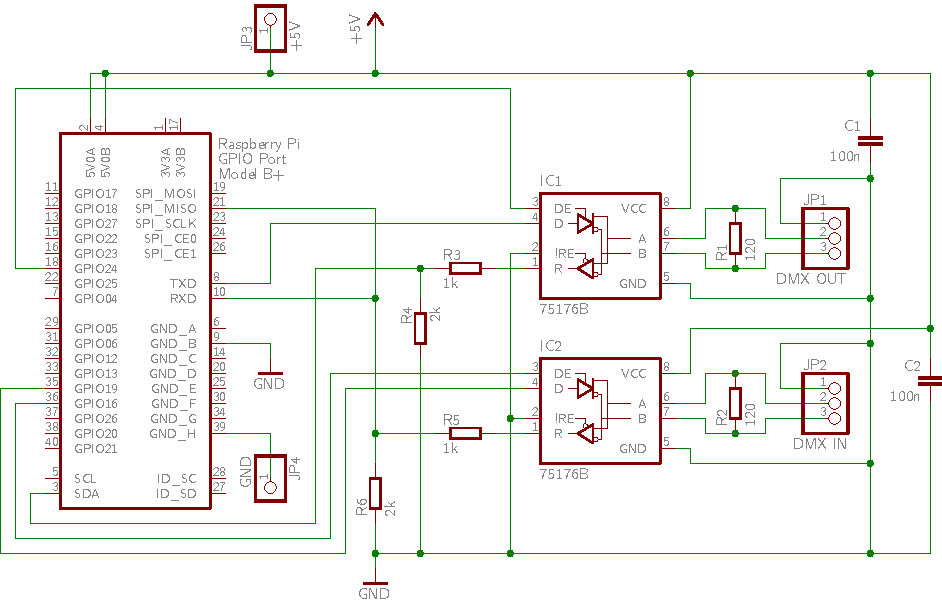
\includegraphics[width=1.00000\textwidth]{Bilder/extension-board-schematic.pdf}
\caption[Extension board schematic]{Extension board schematic. See
\gls{eagle:extension-board.sch}.}\label{fig:extension-board-schematic}
\end{figure}

The schematic is designed such that the \emph{receive} (\emph{R}),
\emph{drive} (\emph{D}) and \emph{drive enable} (\emph{DE}) pins of both
transceiver chips \emph{IC1} and \emph{IC2} -- not just one direction
for each chip -- are connected to the Raspberry Pi. Currently, only one
direction for each chip is supported, but this design allows
bidirectional use of the chips in the future (see \cref{sec:outlook}).
The negated \emph{receive enable} (\emph{!RE}) pin is hard-wired to
ground (\emph{GND}) to enable receiving, as this cannot cause harm to
data transmission.

Received data at the \emph{R} pins are forwarded to the GPIO pins via
voltage dividers (resistors \emph{R3}/\emph{R4} and \emph{R5}/\emph{R6})
to reduce the 5V output signal to the allowed 3.3V for Raspberry Pi's
inputs. \emph{IC2}'s received data (of the DMX input line) additionally
to SPI's \emph{MISO} (\emph{Master In, Slave Out}) pin go also into
UART's \emph{RXD} (receive) pin as that was my first try to make
receiving DMX data on the Raspberry Pi work. \emph{IC1}'s received data
(of the DMX output line) go into the \emph{SDA} pin to keep the option
open to use the \(I^2C\) bus to parse data there; otherwise it can be
used as a simple GPIO pin.

Resistors \emph{R1} and \emph{R2} are DMX termination resistors as
defined in the \protect\hyperlink{sec:dmx-electrical}{DMX standard}.
Both chips' supply voltage (\emph{VCC}) pins are connected to ground via
small capacitors (\emph{C1} and \emph{C2}) to mitigate voltage peaks of
the power supply.

All other parts in the schematic are plug connectors; \emph{JP1} and
\emph{JP2} go to the DMX XLR connectors, \emph{JP3} and \emph{JP4} allow
an external voltage supply to power the Raspberry Pi through the
extension board instead of the onboard micro USB port.

\glsadd[format=(]{eagle:extension-board.brd}This schematic was then
transformed into a two-sided layout that can either be printed to create
a \emph{PCB} (printed circuit board) or soldered manually on a drilled
board, which I did. The layout is shown in
\cref{fig:extension-board-layout}, the finished board in
\cref{fig:extension-board-photos}.\glsadd[format=)]{eagle:extension-board.sch}

\begin{figure}
\centering
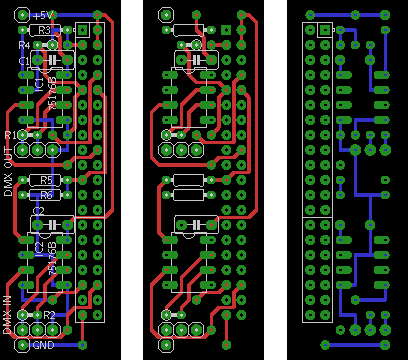
\includegraphics[width=0.75000\textwidth]{Bilder/extension-board-layout.pdf}
\caption[Extension board layout]{Extension board layout. See \gls{eagle:extension-board.brd}.
Complete view, top view without labels, bottom view without labels
(mirrored).}\label{fig:extension-board-layout}
\end{figure}

\glsadd[format=)]{eagle:extension-board.brd}\vspace{-1.2\baselineskip}

\begin{figure}
\centering
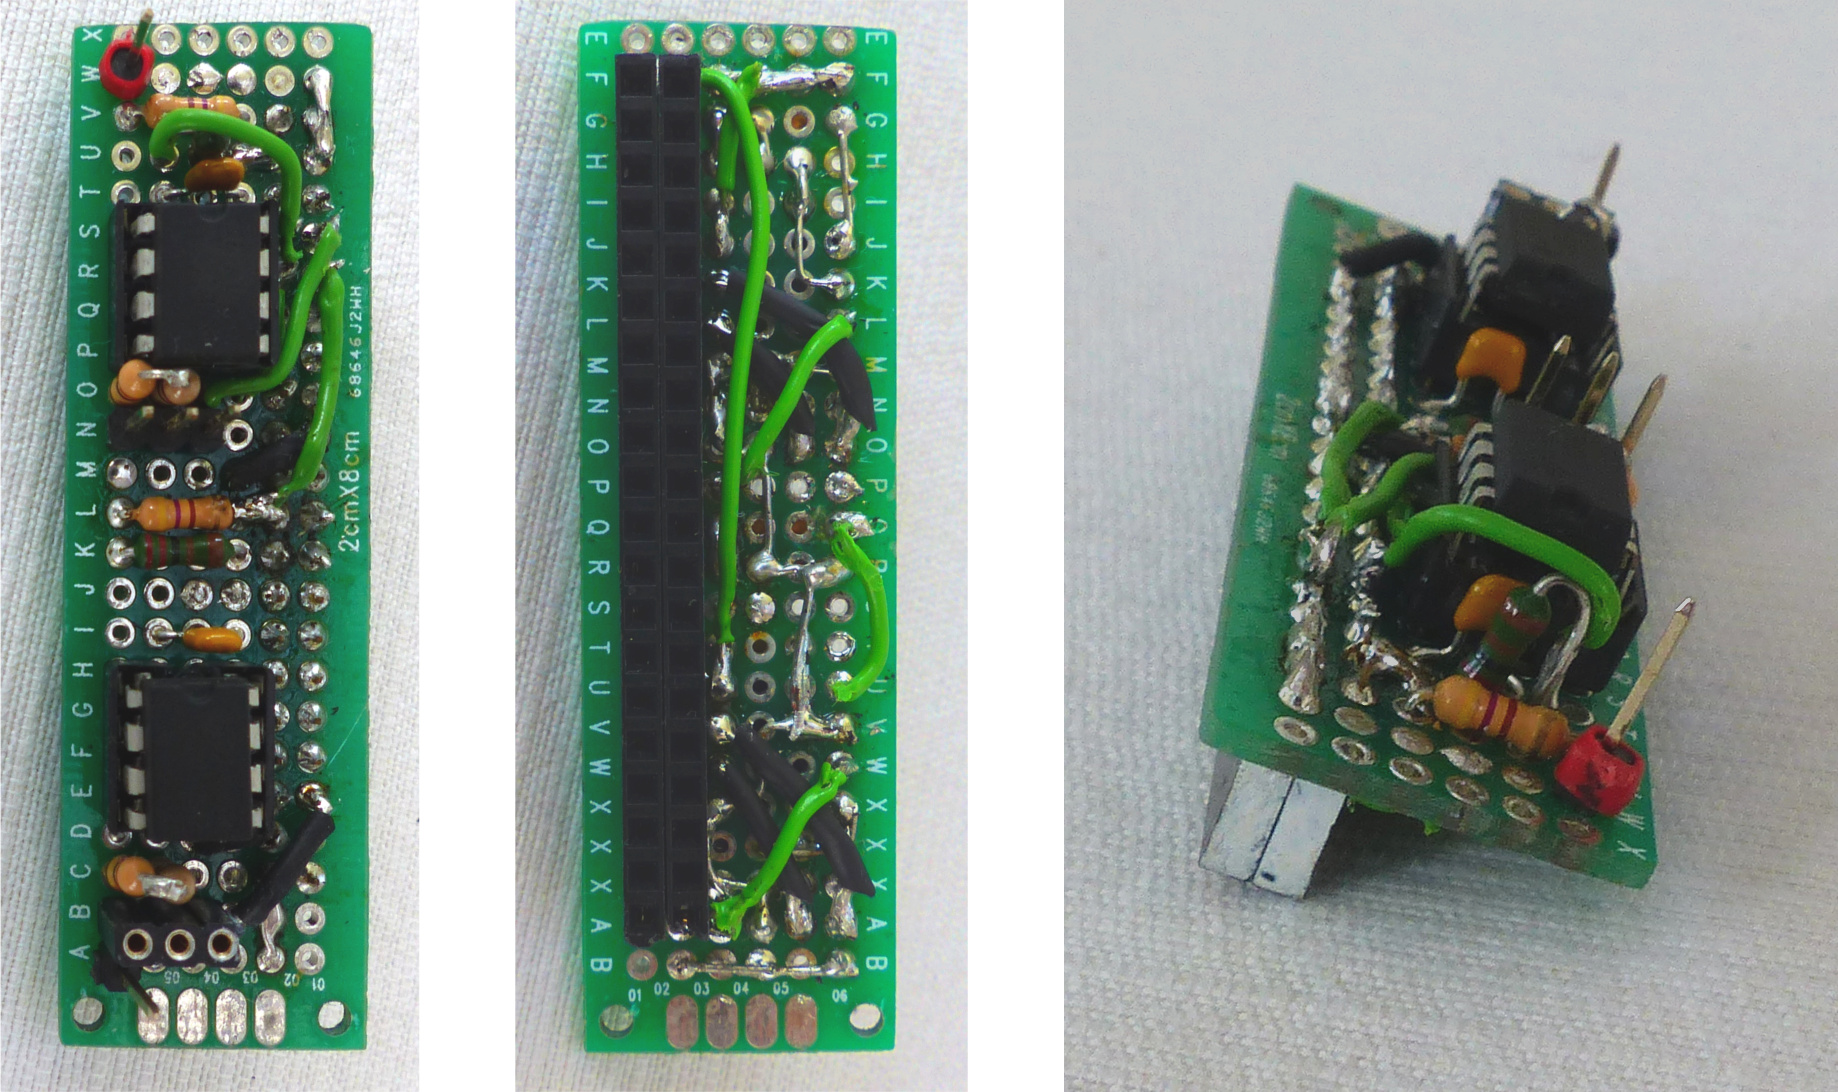
\includegraphics[width=1.00000\textwidth]{Bilder/extension-board-photos.jpg}
\caption[The finished extension board]{The finished extension board. Top view, bottom view, side
view.}\label{fig:extension-board-photos}
\end{figure}

After installing the extension board on Raspberry Pi's GPIO pins,
fixtures connected via \emph{IC1}'s DMX line can be controlled by
changing an OLA universe's channel values in the web interface. The UART
output port just has to be patched to that universe.

In an earlier version, termination resistors were missing, which
resulted in an increased number of transmission errors. Also, both
transceiver chips' \emph{Drive enable} pin were hard-wired to
\emph{VCC}. Thus, whenever the receiver chip (\emph{IC2}) was connected
to a DMX line with another DMX source, it always tried to pull the bus
to \colorbox{WhiteSmoke}{\lstinline!low!} and eventually broke down.

\section{Implementation of the DMXCreator 512 Basic protocol as OLA USB
sub-plugin}\label{sec:ola-dmxcreator-plugin}

The second DMX output port shall be provided by the \emph{DMXCreator 512
Basic} USB-to-DMX adapter\footnote{\url{http://www.dmx512.ch/512.html}}.
It is only officially supported by VXCO's Windows lighting software
\emph{DMXCreator} \citep{vxco-dmxcreator-manual}. To make it usable in
OLA, its protocol must be reverse engineered and then re-implemented as
an extension for the \protect\hyperlink{sec:ola-usb-plugin}{USB DMX
Plugin}.

\subsection{Reverse engineering the protocol with
Wireshark}\label{reverse-engineering-the-protocol-with-wireshark}

\glsadd[format=(]{dmxcreator.pcap}To capture the traffic between the
DMXCreator software and USB adapter, I installed the network analyzer
software \emph{Wireshark} with USB support on Windows\footnote{Instructions:
  \url{https://wiki.wireshark.org/CaptureSetup/USB}} and went through
the steps in \cref{tbl:dmxcreator-wireshark-procedure}. By investigating
the resulting capture file \gls{dmxcreator.pcap}, I found out the
following:

\begin{enumerate}
\def\labelenumi{\arabic{enumi}.}
\tightlist
\item
  Only when the source DMX data changes (e.g.~while fading a slider),
  USB traffic can be observed. The adapter generates a DMX signal with a
  valid refresh rate itself. This was verified by unplugging power of a
  connected fixture, which instantly reset to the correct color when it
  was plugged in again.
\item
  For every DMX data change, one packet with a constant byte string is
  sent to USB endpoint \colorbox{WhiteSmoke}{\lstinline!0x01!} of the device and then either
  one or two data packets (with 256 bytes of payload each) are sent to
  endpoint \colorbox{WhiteSmoke}{\lstinline!0x02!}:

  \begin{enumerate}
  \def\labelenumii{\alph{enumii})}
  \tightlist
  \item
    If the change occurs in the first half of the universe (channels 1
    to 256), the byte string is
    \colorbox{WhiteSmoke}{\lstinline!0x80 0x01 0x00 0x00 0x00 0x01!} and only one data packet
    is sent.
  \item
    If the change occurs in the second half (channels 257 to 512), the
    byte string is \colorbox{WhiteSmoke}{\lstinline!0x80 0x01 0x00 0x00 0x00 0x02!} and two
    data packets are sent.
  \end{enumerate}
\item
  The data packets' payload consists of half a universe's DMX channel
  values as one byte string. Hence, two data packets are needed if the
  changed channel is located in the second half.
\item
  The USB device's vendor ID is \colorbox{WhiteSmoke}{\lstinline!0x0a30!}, its product ID is
  \colorbox{WhiteSmoke}{\lstinline!0x0002!} (included in packet 88; can also be retrieved by
  running \colorbox{WhiteSmoke}{\lstinline!lsusb!} on Linux).
\end{enumerate}

\hypertarget{tbl:dmxcreator-wireshark-procedure}{}
\begin{longtable}[]{@{}rlc@{}}
\caption[Procedure for
capturing DMXCreator's USB communication protocol]{\label{tbl:dmxcreator-wireshark-procedure}Procedure for
capturing DMXCreator's USB communication protocol. The \emph{pcap
packets} column corresponds to the packets in \gls{dmxcreator.pcap} that
were captured during each step. }\tabularnewline
\toprule
\begin{minipage}[b]{0.05\columnwidth}\raggedleft\strut
\#\strut
\end{minipage} & \begin{minipage}[b]{0.74\columnwidth}\raggedright\strut
Step\strut
\end{minipage} & \begin{minipage}[b]{0.13\columnwidth}\centering\strut
\emph{pcap} packets\strut
\end{minipage}\tabularnewline
\midrule
\endfirsthead
\toprule
\begin{minipage}[b]{0.05\columnwidth}\raggedleft\strut
\#\strut
\end{minipage} & \begin{minipage}[b]{0.74\columnwidth}\raggedright\strut
Step\strut
\end{minipage} & \begin{minipage}[b]{0.13\columnwidth}\centering\strut
\emph{pcap} packets\strut
\end{minipage}\tabularnewline
\midrule
\endhead
\begin{minipage}[t]{0.05\columnwidth}\raggedleft\strut
1.\strut
\end{minipage} & \begin{minipage}[t]{0.74\columnwidth}\raggedright\strut
Start to capture USB traffic with Wireshark.\strut
\end{minipage} & \begin{minipage}[t]{0.13\columnwidth}\centering\strut
0 -- 26\strut
\end{minipage}\tabularnewline
\begin{minipage}[t]{0.05\columnwidth}\raggedleft\strut
2.\strut
\end{minipage} & \begin{minipage}[t]{0.74\columnwidth}\raggedright\strut
Plug in the DMXCreator 512 Basic USB adapter.\strut
\end{minipage} & \begin{minipage}[t]{0.13\columnwidth}\centering\strut
27 -- 97\strut
\end{minipage}\tabularnewline
\begin{minipage}[t]{0.05\columnwidth}\raggedleft\strut
3.\strut
\end{minipage} & \begin{minipage}[t]{0.74\columnwidth}\raggedright\strut
Start the DMXCreator software.\strut
\end{minipage} & \begin{minipage}[t]{0.13\columnwidth}\centering\strut
98 -- 103\strut
\end{minipage}\tabularnewline
\begin{minipage}[t]{0.05\columnwidth}\raggedleft\strut
4.\strut
\end{minipage} & \begin{minipage}[t]{0.74\columnwidth}\raggedright\strut
Patch \emph{eurolite LED PAR-64 RGB Spot} fixture (5 channels: Red,
Green, Blue, Dimmer, Flash) to DMX address 1.\strut
\end{minipage} & \begin{minipage}[t]{0.13\columnwidth}\centering\strut
\strut
\end{minipage}\tabularnewline
\begin{minipage}[t]{0.05\columnwidth}\raggedleft\strut
5.\strut
\end{minipage} & \begin{minipage}[t]{0.74\columnwidth}\raggedright\strut
Patch another \emph{eurolite LED PAR-64 RGB Spot} fixture to DMX address
367.\strut
\end{minipage} & \begin{minipage}[t]{0.13\columnwidth}\centering\strut
\strut
\end{minipage}\tabularnewline
\begin{minipage}[t]{0.05\columnwidth}\raggedleft\strut
6.\strut
\end{minipage} & \begin{minipage}[t]{0.74\columnwidth}\raggedright\strut
Go to main window.\strut
\end{minipage} & \begin{minipage}[t]{0.13\columnwidth}\centering\strut
104 -- 106\strut
\end{minipage}\tabularnewline
\begin{minipage}[t]{0.05\columnwidth}\raggedleft\strut
7.\strut
\end{minipage} & \begin{minipage}[t]{0.74\columnwidth}\raggedright\strut
Slowly fade the first fixture's \emph{Red} channel (DMX channel 1) down
from 255 to 0.\strut
\end{minipage} & \begin{minipage}[t]{0.13\columnwidth}\centering\strut
107 -- 260\strut
\end{minipage}\tabularnewline
\begin{minipage}[t]{0.05\columnwidth}\raggedleft\strut
8.\strut
\end{minipage} & \begin{minipage}[t]{0.74\columnwidth}\raggedright\strut
Slowly fade the second fixture's \emph{Blue} channel (DMX channel 369)
down from 255 to 86.\strut
\end{minipage} & \begin{minipage}[t]{0.13\columnwidth}\centering\strut
261 -- 386\strut
\end{minipage}\tabularnewline
\begin{minipage}[t]{0.05\columnwidth}\raggedleft\strut
9.\strut
\end{minipage} & \begin{minipage}[t]{0.74\columnwidth}\raggedright\strut
Slowly fade the second fixture's \emph{Green} channel (DMX channel 368)
down from 255 to 0.\strut
\end{minipage} & \begin{minipage}[t]{0.13\columnwidth}\centering\strut
387 -- 224\strut
\end{minipage}\tabularnewline
\begin{minipage}[t]{0.05\columnwidth}\raggedleft\strut
10.\strut
\end{minipage} & \begin{minipage}[t]{0.74\columnwidth}\raggedright\strut
End capturing.\strut
\end{minipage} & \begin{minipage}[t]{0.13\columnwidth}\centering\strut
\strut
\end{minipage}\tabularnewline
\bottomrule
\end{longtable}

\glsadd[format=)]{dmxcreator.pcap}\vspace{-1.2\baselineskip}

\subsection{Extending OLA's USB DMX
Plugin}\label{extending-olas-usb-dmx-plugin}

The reverse-engineered protocol now had to be incorporated into OLA's
\protect\hyperlink{sec:ola-usb-plugin}{USB DMX Plugin}. Since this
plugin does not depend on Raspberry Pi's embedded hardware, development
could happen completely on my more powerful work computer to speed up
build times.

\emph{Note:} All code blocks in this section can be found unshortened in
OLA's GitHub pull request 1136\footnote{\url{https://github.com/OpenLightingProject/ola/pull/1136/files}}.

First, the user starting \colorbox{WhiteSmoke}{\lstinline!olad!} has to be given permissions to
communicate with the USB adapter. This can be achieved by adding the
following rule to the udev rules from \cref{sec:usb-configuration} in
\colorbox{WhiteSmoke}{\lstinline!/etc/udev/rules.d/10-ola.rules!} and reloading the rules. It
allows all members of the \emph{plugdev} group access to USB devices
identified by the given vendor and product IDs.

\begin{lstlisting}[numbers=left, style=myBash, firstnumber=19]
# udev rules for the DMXCreator 512 Basic device
SUBSYSTEM=="usb|usb_device", ACTION=="add", ATTRS{idVendor}=="0a30", ATTRS{idProduct}=="0002", GROUP="plugdev"
\end{lstlisting}

I also added the rule to OLA's \gls{ola.udev} file to have it included
in released OLA \colorbox{WhiteSmoke}{\lstinline!.deb!} packages. When installing these, the
rules gets extracted to the correct location.

\paragraph{DMXCreator512BasicFactory (factory
class)}\label{dmxcreator512basicfactory-factory-class}

\glsadd[format=(]{usbdmx:DMXCreator512BasicFactory.cpp}For creating a
new sub-plugin of the USB DMX Plugin, I followed its developer
information document\footnote{\url{https://github.com/OpenLightingProject/ola/blob/master/plugins/usbdmx/README.developer.md}}.
Every sub-plugin has a \emph{factory} class, whose
\colorbox{WhiteSmoke}{\lstinline!DeviceAdded!} method is called whenever a new USB device is
found. This method is expected to return \colorbox{WhiteSmoke}{\lstinline!false!} if the device
should not or cannot be claimed by this sub-plugin. In
\emph{DMXCreator}'s case, the only identifying attributes of the USB
adapter are its vendor and product IDs.

\begin{lstlisting}[numbers=left, style=myCpp, firstnumber=36, caption={[Excerpt from \glsfont{DMXCreator512BasicFactory.cpp}]Excerpt from \gls{usbdmx:DMXCreator512BasicFactory.cpp}.}]
const uint16_t DMXCreator512BasicFactory::VENDOR_ID = 0x0a30;
const uint16_t DMXCreator512BasicFactory::PRODUCT_ID = 0x0002;

bool DMXCreator512BasicFactory::DeviceAdded(
    WidgetObserver *observer,
    libusb_device *usb_device,
    const struct libusb_device_descriptor &descriptor) {
  if (descriptor.idVendor != VENDOR_ID || descriptor.idProduct != PRODUCT_ID) {
    return false;
  }

  LibUsbAdaptor::DeviceInformation info;
  if (!m_adaptor->GetDeviceInfo(usb_device, descriptor, &info)) {
    return false;
  }

  OLA_INFO << "Found a new DMXCreator 512 Basic device";
\end{lstlisting}

The USB adapter does not return a serial number, so because it is not
possible to distinguish between different devices, only one at a time is
supported.

\begin{lstlisting}[numbers=left, style=myCpp, firstnumber=58]
  if (info.serial.empty()) {
    if (m_missing_serial_number) {
      OLA_WARN << "We can only support one device without a serial number.";
      return false;
    } else {
      m_missing_serial_number = true;
    }
  }
\end{lstlisting}

In the case that the device \emph{should} be claimed, the method creates
a new widget instance, passes it to \colorbox{WhiteSmoke}{\lstinline!BaseWidgetFactory!}'s
\colorbox{WhiteSmoke}{\lstinline!AddWidget!} method (located in \emph{WidgetFactory.h}), which
tries to initialize it, and returns the result. OLA supports detecting
\emph{hot-plugged} devices (i.e.~devices plugged in after OLA was
started) in the default asynchronous mode of the underlying
\colorbox{WhiteSmoke}{\lstinline!libusb!} library, but a fallback version using
\colorbox{WhiteSmoke}{\lstinline!libusb!}'s synchronous methods shall be implemented as well.
Thus, two classes \colorbox{WhiteSmoke}{\lstinline!AsynchronousDMXCreator512Basic!} and
\colorbox{WhiteSmoke}{\lstinline!SynchronousDMXCreator512Basic!} are implemented as child
classes of the widget class
\colorbox{WhiteSmoke}{\lstinline!DMXCreator512Basic!}.\glsadd[format=)]{usbdmx:DMXCreator512BasicFactory.cpp}

\paragraph{DMXCreator512Basic (widget
class)}\label{dmxcreator512basic-widget-class}

\glsadd[format=(]{usbdmx:DMXCreator512Basic.cpp}The protocol allows
sending a whole universe (instead of only the first half), thus I
decided to always use this method. In
\gls{usbdmx:DMXCreator512Basic.cpp}, I declared a constant array with
the bytes which should be sent to USB endpoint \colorbox{WhiteSmoke}{\lstinline!0x01!}.

\begin{lstlisting}[numbers=left, style=myCpp, firstnumber=55, caption={[Excerpt from \glsfont{DMXCreator512Basic.cpp}]Excerpt from \gls{usbdmx:DMXCreator512Basic.cpp}.}]
// if we only wanted to send the first half of the universe, the last byte would
// be 0x01
static const uint8_t status_buffer[6] = {
  0x80, 0x01, 0x00, 0x00, 0x00, 0x02
};
\end{lstlisting}

Both the synchronous and asynchronous implementations of
\colorbox{WhiteSmoke}{\lstinline!DMXCreator512Basic!} use the \emph{Facade} software pattern,
i.e.~method calls to the widget class are passed through to a child
class of \colorbox{WhiteSmoke}{\lstinline!ThreadedUsbSender!} or \colorbox{WhiteSmoke}{\lstinline!AsyncUsbSender!},
respectively. I explain my approach to implementing the synchronous
version here because it is a bit easier to understand. The asynchronous
version provides the same functionality while using asynchronous
\colorbox{WhiteSmoke}{\lstinline!libusb!} methods and callback functions.

For initialization, the USB device must be opened and claimed. With the
resulting device handle, the \colorbox{WhiteSmoke}{\lstinline!ThreadedUsbSender!} child class
can be instantiated and a pointer of it is saved in the instance
variable \colorbox{WhiteSmoke}{\lstinline!m_sender!}.

\begin{lstlisting}[numbers=left, style=myCpp, firstnumber=160]
bool SynchronousDMXCreator512Basic::Init() {
  libusb_device_handle *usb_handle;

  bool ok = m_adaptor->OpenDeviceAndClaimInterface(
      m_usb_device, 0, &usb_handle);
  if (!ok) {
    return false;
  }

  std::auto_ptr<DMXCreator512BasicThreadedSender> sender(
      new DMXCreator512BasicThreadedSender(m_adaptor, m_usb_device,
                                           usb_handle));
  if (!sender->Start()) {
    return false;
  }
  m_sender.reset(sender.release());
  return true;
}
\end{lstlisting}

Whenever new DMX data shall be sent via this USB adapter, the widget's
\colorbox{WhiteSmoke}{\lstinline!SendDMX!} method is called, which just forwards the
\colorbox{WhiteSmoke}{\lstinline!DmxBuffer!} object to \colorbox{WhiteSmoke}{\lstinline!m_sender!} if it is already
available (i.e.~if the \colorbox{WhiteSmoke}{\lstinline!Init!} function was called correctly
before), whose infinite loop then in turn calls
\colorbox{WhiteSmoke}{\lstinline!TransmitBuffer!} in the next iteration.

\begin{lstlisting}[numbers=left, style=myCpp, firstnumber=179]
bool SynchronousDMXCreator512Basic::SendDMX(const DmxBuffer &buffer) {
  return m_sender.get() ? m_sender->SendDMX(buffer) : false;
}
\end{lstlisting}

In \colorbox{WhiteSmoke}{\lstinline!TransmitBuffer!}, the provided \colorbox{WhiteSmoke}{\lstinline!DmxBuffer!} first
is compared with the last transmitted one. If they are the same, nothing
needs to be transmitted at all.

\begin{lstlisting}[numbers=left, style=myCpp, firstnumber=96]
bool DMXCreator512BasicThreadedSender::TransmitBuffer(
    libusb_device_handle *handle, const DmxBuffer &buffer) {

  if (m_dmx_buffer == buffer) {
    // no need to update -> sleep 50µs to avoid timeout errors
    usleep(50);
    return true;
  }

  m_dmx_buffer = buffer;
\end{lstlisting}

Else, both halves of the universe are copied into
\colorbox{WhiteSmoke}{\lstinline!m_universe_lower!} and \colorbox{WhiteSmoke}{\lstinline!m_universe_upper!}. If the
provided \colorbox{WhiteSmoke}{\lstinline!DmxBuffer!} does not contain all 512 channels (the
\colorbox{WhiteSmoke}{\lstinline!length!} variable gets set to the number of copied channels),
the rest is filled up with zeros.

\begin{lstlisting}[numbers=left, style=myCpp, firstnumber=107]
  unsigned int length = CHANNELS_PER_PACKET;
  m_dmx_buffer.Get(m_universe_data_lower, &length);
  memset(m_universe_data_lower + length, 0, CHANNELS_PER_PACKET - length);

  length = CHANNELS_PER_PACKET;
  m_dmx_buffer.GetRange(CHANNELS_PER_PACKET, m_universe_data_upper, &length);
  memset(m_universe_data_upper + length, 0, CHANNELS_PER_PACKET - length);
\end{lstlisting}

Afterwards, \colorbox{WhiteSmoke}{\lstinline!status_buffer!} is sent to USB endpoint
\colorbox{WhiteSmoke}{\lstinline!0x01!} and both halves are consecutively sent to endpoint
\colorbox{WhiteSmoke}{\lstinline!0x02!}. If any operation fails, \colorbox{WhiteSmoke}{\lstinline!false!} is returned,
so that the thread stops and the device handle gets closed.

\begin{lstlisting}[numbers=left, style=myCpp, firstnumber=115]
  bool r = BulkTransferPart(handle, ENDPOINT_1, status_buffer,
                            sizeof(status_buffer), "status");
  if (!r) {
    return false;
  }

  r = BulkTransferPart(handle, ENDPOINT_2, m_universe_data_lower,
                       CHANNELS_PER_PACKET, "lower data");
  if (!r) {
    return false;
  }

  r = BulkTransferPart(handle, ENDPOINT_2, m_universe_data_upper,
                       CHANNELS_PER_PACKET, "upper data");
  return r;
}
\end{lstlisting}

~\glsadd[format=)]{usbdmx:DMXCreator512Basic.cpp}

\paragraph{Integration}\label{integration}

At several locations, the new classes had to be integrated into the USB
DMX Plugin. However, the required snippets are very similar to all
existing sub-plugins, hence, I will not include them here, but only
provide a list of changed files and functions for reference:

\begin{itemize}
\tightlist
\item
  \gls{usbdmx:AsyncPluginImpl.cpp}:\\
  instantiated factory class in \colorbox{WhiteSmoke}{\lstinline!Start!} method; overloaded
  \colorbox{WhiteSmoke}{\lstinline!NewWidget!} method
\item
  \gls{usbdmx:AsyncPluginImpl.h}:\\
  overloaded \colorbox{WhiteSmoke}{\lstinline!NewWidget!} method
\item
  \gls{usbdmx:SyncPluginImpl.cpp}:\\
  instantiated factory class in constructor; overloaded
  \colorbox{WhiteSmoke}{\lstinline!NewWidget!} method
\item
  \gls{usbdmx:SyncPluginImpl.h}:\\
  overloaded \colorbox{WhiteSmoke}{\lstinline!NewWidget!} method
\item
  \gls{usbdmx:SyncronizedWidgetObserver.h} {[}sic{]}\footnote{I raised
    issue
    \href{https://github.com/OpenLightingProject/ola/issues/1331}{\#1331}
    on GitHub to correct the typing error.}:\\
  overloaded \colorbox{WhiteSmoke}{\lstinline!NewWidget!} method
\item
  \gls{usbdmx:WidgetFactory.h}:\\
  overloaded virtual \colorbox{WhiteSmoke}{\lstinline!NewWidget!} method
\end{itemize}

Additionally, the USB adapter was included in
\gls{usbdmx:UsbDmxPlugin.cpp}'s plugin description\footnote{Today, after
  changes in OLA's plugin structure, the plugin description is located
  in \emph{README.md} and read~in from there.} and the new files had to
be added to \gls{usbdmx:Makefile.mk} to allow recompiling with
\colorbox{WhiteSmoke}{\lstinline!make!} and \colorbox{WhiteSmoke}{\lstinline!make install!}.

Now, patching the new \emph{DMXCreator 512 Basic USB Device} to a
universe in OLA's web interface and sending DMX data through it is
working as expected.

The new code was merged back into OLA's project repository on
GitHub\footnote{\url{https://github.com/OpenLightingProject/ola/pull/1136}},
after improving my initial version together with the project's main
developers Peter Newman and Simon Newton.

\section{Implementation of the OLA Native SPI DMX
Plugin}\label{sec:ola-spidmx-plugin}

Two output ports are provided by the UART and USB DMX plugins, the input
port is yet to be implemented. In this section I briefly describe my
first two approaches and why they failed. Afterwards, the working
solution with SPI is explained in detail.

\subsection{Insufficiency of Raspberry Pi's UART
input}\label{sec:uart-insufficiency}

My first idea was to extend the UART plugin to also support DMX input.
This seemed perfect since the UART and DMX protocols are so similar and
very little software overhead would be needed.

However, there is a big catch: Receiving and recognizing the BREAK
signal is very difficult because it is just forwarded to the application
as a null byte and thus indistinguishable from data channels that are
just set to zero. There are options in the \colorbox{WhiteSmoke}{\lstinline!termios!} C
interface's \colorbox{WhiteSmoke}{\lstinline!c_iflag!} input flags to change this:

\begin{lstlisting}[morekeywords={BRKINT, IGNBRK, PARMRK, INPCK, IGNPAR, ISTRIP}, caption={[Excerpt from the \emph{termios} man page]Excerpt from the \emph{termios} man page. Note that octal {\textbackslash}377 is 255 in decimal.}]
BRKINT If IGNBRK is set, a BREAK is ignored.  If it is not set but
       BRKINT is set, then a BREAK causes the input and output queues
       to be flushed, and if the terminal is the controlling terminal
       of a foreground process group, it will cause a SIGINT to be
       sent to this foreground process group.  When neither IGNBRK
       nor BRKINT are set, a BREAK reads as a null byte ('\0'),
       except when PARMRK is set, in which case it reads as the
       sequence \377 \0 \0.

IGNPAR Ignore framing errors and parity errors.

PARMRK If this bit is set, input bytes with parity or framing errors
       are marked when passed to the program.  This bit is meaningful
       only when INPCK is set and IGNPAR is not set.  The way erro-
       neous bytes are marked is with two preceding bytes, \377 and
       \0.  Thus, the program actually reads three bytes for one
       erroneous byte received from the terminal.  If a valid byte
       has the value \377, and ISTRIP (see below) is not set, the
       program might confuse it with the prefix that marks a parity
       error.  Therefore, a valid byte \377 is passed to the program
       as two bytes, \377 \377, in this case.

       If neither IGNPAR nor PARMRK is set, read a character with a
       parity error or framing error as \0.

INPCK  Enable input parity checking.

ISTRIP Strip off eighth bit.
\end{lstlisting}

However, regardless of which settings I tried, after some time only
random data bytes were decoded. The UART seemed to be confused by the
frequent BREAKs.

I was unable to figure out where this issue arose from because I could
not verify if the signal was captured by the UART correctly. So I
decided to look for a way to receive data that permits access to the
``raw'' DMX signal, as this would potentially be a more stable approach.
It would require implementing parsing myself but thereby also give me
full control over it.

\subsection{Bit bang reading with pigpio
library}\label{bit-bang-reading-with-pigpio-library}

The next idea was to constantly poll one GPIO pin's value and getting
the raw signal that way. This technique is known as ``bit bang reading''
in the \emph{pigpio} library\footnote{\url{http://abyz.me.uk/rpi/pigpio/cif.html\#gpioSerialReadOpen}}.
I had concerns about the speed and precision of the read process, since
Linux is not a real time operating system and scheduling could delay
read operations so that they already sample the pin when the next bit is
fed in. At 250kbit/s, these delays could already be significant.

Fortunately, \emph{pigpio} provides a diagnose tool called
\emph{piscope} that displays the bit banged signal. I generated DMX data
with an external DMX interface and inspected the signal captured by
\emph{piscope}. An example capture image together with the expected
signal can be seen in \cref{fig:piscope-vs-spi}.

\begin{figure}
\centering

\includegraphics[width=1.00000\textwidth]{Bilder/piscope-vs-spi.pdf}
\caption[\emph{pigpio} ``bit bang read'' signal shown in \emph{piscope}
(top) versus sent data]{\emph{pigpio} ``bit bang read'' signal shown in \emph{piscope}
(top) versus sent data. The sent channel values are 255, 0, 0, 127, 0,
0, 255, 255, 0, 0, \ldots{}}\label{fig:piscope-vs-spi}
\end{figure}

This revealed that often a short pulse, i.e.~a quick change from
\colorbox{WhiteSmoke}{\lstinline!low!} to \colorbox{WhiteSmoke}{\lstinline!high!} to \colorbox{WhiteSmoke}{\lstinline!low!} or the other way
around, was not visible at all, e.g.~in slot 4 and 7 in
\cref{fig:piscope-vs-spi}. Additionally, sampling seemed to happen once
every 5µs, since slots' stop bits (2 \colorbox{WhiteSmoke}{\lstinline!high!} bits) lasted
sometimes 5µs and sometimes 10µs, but never 8µs as expected.

In conclusion, ``bit bang reading'' a GPIO pin is not sufficiently
accurate for the 250kbit/s DMX signal.

\subsection{Using SPI to sample DMX}\label{using-spi-to-sample-dmx}

An idea I came across in a \emph{Raspberry Pi StackExchange}
answer\footnote{\url{https://raspberrypi.stackexchange.com/a/2044}}
while researching GPIO bit banging speeds was sampling the native SPI
port (see \cref{sec:spi}) for arbitrary DMX data. For this, the DMX line
is connected (via the bus transceiver) to Raspberry Pi's \emph{MISO}
(\emph{Master In, Slave Out}) pin, the other SPI pins are left
unconnected. The intention is that SPI is designed for much higher
speeds than UART, so a stable clock frequency is important.
Unfortunately, not many details were provided in that post, and it seems
to be a very uncommon technique, so I had to figure out most steps
myself.

Raspberry Pi's SPI controller (acting as SPI master) has a core
frequency of 250MHz that can be divided by any even number\footnote{According
  to the BCM2835 manual \citep{broadcom-bcm2835}, only powers of two can
  be used as clock divider, but this is incorrect according to
  \url{https://raspberrypi.stackexchange.com/a/3444} and testing by
  myself.}. The goal is to sample the connected DMX signal 8 times per
bit to have enough tolerance if sometimes the sample time falls exactly
on an edge, so the required sample frequency is 250kbit/s · 8/bit =
2MHz. The required clock divider 250MHz / 2MHz = 125 is odd, so 124 will
be used instead (odd divisors are rounded down) and parsing of the
sampled bits must be flexible enough to account for this inaccuracy.
However, since a valid DMX receiver has to accept any signal with a bit
rate of 245kbit/s to 255kbit/s (see \cref{sec:dmx-protocol}),
flexibility must be ensured anyway.

\begin{align*}
f_{eff} = \frac{250\text{MHz}}{124} &\approx 2.02\text{MHz}\\[3pt]
\frac{f_{eff}}{245\text{kbit/s}} &\approx \frac{8.23\text{ sampled bits}}{\text{DMX bit}}\\[3pt]
\frac{f_{eff}}{250\text{kbit/s}} &\approx \frac{8.06\text{ sampled bits}}{\text{DMX bit}}\\[3pt]
\frac{f_{eff}}{255\text{kbit/s}} &\approx \frac{7.91\text{ sampled bits}}{\text{DMX bit}}
\end{align*}

\subsubsection{Enabling SPI}\label{enabling-spi}

Enabling SPI can be done with \colorbox{WhiteSmoke}{\lstinline!raspi-config!}. To increase the
buffer size (i.e.~the number of bytes that can be received/transmitted
in one operation), \colorbox{WhiteSmoke}{\lstinline!spidev.bufsiz=65536!} should be added to
the kernel options in \colorbox{WhiteSmoke}{\lstinline!/boot/cmdline.txt!}. After a reboot, the
value returned by \colorbox{WhiteSmoke}{\lstinline!cat /sys/module/spidev/parameters/bufsiz!}
should be the requested 65536.

\emph{Note:} Since there is much contradicting information available
online, I want to clarify: In newer firmware versions, no additional
steps (like manually enabling a kernel module or blacklisting another)
are needed.

To test the configuration, the \emph{MISO} and \emph{MOSI} pins can be
wired together for a \emph{loopback} test:

\begin{lstlisting}[style=myBash, morekeywords={wget, gcc}]
wget https://raw.githubusercontent.com/raspberrypi/linux/rpi-3.10.y/Documentation/spi/spidev_test.c
gcc -o spidev_test spidev_test.c
./spidev_test --device /dev/spidev0.0 --speed 2000000
\end{lstlisting}

Output should look like the following.

\begin{lstlisting}
spi mode: 0
bits per word: 8
max speed: 2000000 Hz (2000 KHz)

FF FF FF FF FF FF
40 00 00 00 00 95
FF FF FF FF FF FF
FF FF FF FF FF FF
FF FF FF FF FF FF
DE AD BE EF BA AD
F0 0D
\end{lstlisting}

Additionally, I ran the test while connecting the \emph{MISO} pin to
either +3.3V, ground, or leaving it unconnected. As expected, the output
was \colorbox{WhiteSmoke}{\lstinline!FF!}s only, \colorbox{WhiteSmoke}{\lstinline!00!}s only and again \colorbox{WhiteSmoke}{\lstinline!00!}s
only, respectively.

\subsubsection{Receiving DMX data}\label{receiving-dmx-data}

\glsadd[format=(]{spi-receive.c}Based on the loopback test program
above, I wrote \gls{spi-receive.c}, which reads in 8192 bytes\footnote{On
  Raspberry Pi, \emph{spidev}'s buffer size is 4096 bytes by default.
  Because this limit is too low (see end of \cref{sec:spidmx-wrapping}),
  its maximum size was increased to 65536 in the previous section.} four
times from the SPI MISO bus and outputs them in binary format to the
console. As the loopback test code and the existing SPI Plugin (see
\cref{sec:ola-spi-plugin}) do too, it uses the \colorbox{WhiteSmoke}{\lstinline!spidev!}
interface, which enables SPI communication from user space (not as part
of the kernel).

A single SPI transfer with \colorbox{WhiteSmoke}{\lstinline!spidev!} is configured by an
\colorbox{WhiteSmoke}{\lstinline!spi_ioc_transfer!} struct like shown below. The transfer
itself is then executed with
\colorbox{WhiteSmoke}{\lstinline!ioctl(fd, SPI_IOC_MESSAGE(1), &tr)!}.

\begin{lstlisting}[numbers=left, style=myCpp, firstnumber=43, caption={[Excerpt from \glsfont{spi-receive.c}]Excerpt from \gls{spi-receive.c}.}, label=lst:spi-receive]
  struct spi_ioc_transfer tr = {
    // don't transmit anything
    .tx_buf = 0,

    // save received bytes into `rx` buffer (at appropriate offset)
    .rx_buf = (unsigned long)(rx + BYTES_PER_TRANSFER*offset),

    // bytes to send/receive in this transfer operation
    .len = BYTES_PER_TRANSFER,

    // don't delay after data bytes are sent
    .delay_usecs = delay,

    // overwrite speed temporarily to 2MHz
    .speed_hz = speed,

    // overwrite bits per word temporarily to 8
    .bits_per_word = bits_per_word,
  };
\end{lstlisting}

The \colorbox{WhiteSmoke}{\lstinline!transfer!} function, where the struct above is created and
used to initiate the SPI data transfer, is called four times.
Afterwards, the \colorbox{WhiteSmoke}{\lstinline!printBinary!} function prints the
\colorbox{WhiteSmoke}{\lstinline!rx!} buffer as binary numbers. It uses the
\colorbox{WhiteSmoke}{\lstinline!BYTE_TO_BINARY!} macro to deconstruct bytes into 8 ones and
zeros.

\begin{lstlisting}[numbers=left, style=myCpp, firstnumber=71]
#define BYTE_TO_BINARY_PATTERN "%c %c %c %c %c %c %c %c "
#define BYTE_TO_BINARY(byte)  \
  (byte & 0x80 ? '1' : '0'), \
  (byte & 0x40 ? '1' : '0'), \
  (byte & 0x20 ? '1' : '0'), \
  (byte & 0x10 ? '1' : '0'), \
  (byte & 0x08 ? '1' : '0'), \
  (byte & 0x04 ? '1' : '0'), \
  (byte & 0x02 ? '1' : '0'), \
  (byte & 0x01 ? '1' : '0')
\end{lstlisting}

\glsadd[format=)]{spi-receive.c}\glsadd[format=(]{dmx-spi-data.txt}I
tried the program with an example DMX signal and saved the resulting
binary data to \gls{dmx-spi-data.txt}. Then these data were loaded and
plotted in \emph{GNU Octave}\footnote{\url{https://www.gnu.org/software/octave/}}
with the following commands. A screenshot of the resulting plot is shown
in \cref{fig:octave-spi}.

\begin{lstlisting}[style=myBash, morekeywords={load, stairs, axis}]
load "dmx-spi-data.txt"
data2 = dmx_spi_data(2, :)  # copy 2nd chunk
stairs(data2 * 0.9 + 0.05)  # show square signal
axis([17000 19500 0 1])     # show x values (bits) 17000...19500, y values 0...1
\end{lstlisting}

\begin{figure}
\centering
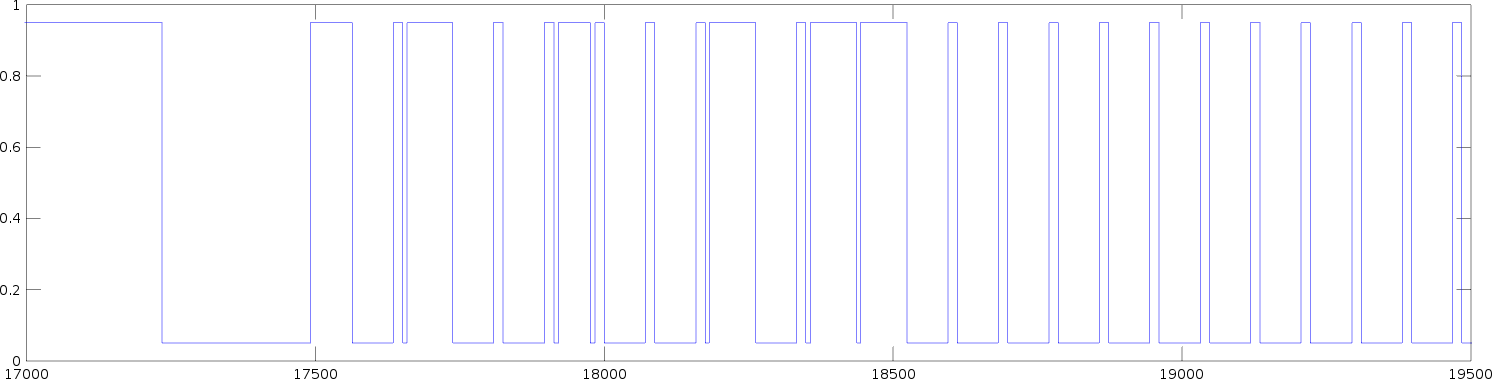
\includegraphics[width=1.00000\textwidth]{Bilder/octave-spi.png}
\caption[Received SPI data (excerpt) plotted with GNU
Octave]{Received SPI data (excerpt) plotted with GNU
Octave.}\label{fig:octave-spi}
\end{figure}

I repeated the procedure multiple times and the plots kept looking very
promising. No short pulses were missed and due to the oversampling, the
timing was also very accurate\footnote{Actually, the ``real'' DMX signal
  that the \emph{piscope} bit banged signal in \cref{fig:piscope-vs-spi}
  was compared against, was a plot of the same data received with SPI.}.
The only problem I noticed was that two consecutive chunks
(i.e.~received in multiple transfer operations) are separated by an
uncaptured gap, even if the \colorbox{WhiteSmoke}{\lstinline!transfer!} calls are right after
each other in the code.

That means that the resulting bytes cannot be parsed as a (possibly
infinitely) long stream of bits, but rather each chunk must be parsed on
its own. As a result, there are chunks that do only contain the start of
a DMX packet, some do only contain the end. These are useless though,
since it is not clear how many channels have been transmitted before.
Thus, the refresh rate is lower for higher channels. The problem is
visualized in
\cref{fig:spi-dmx-chunks}.\glsadd[format=)]{dmx-spi-data.txt}

\begin{figure}
\centering
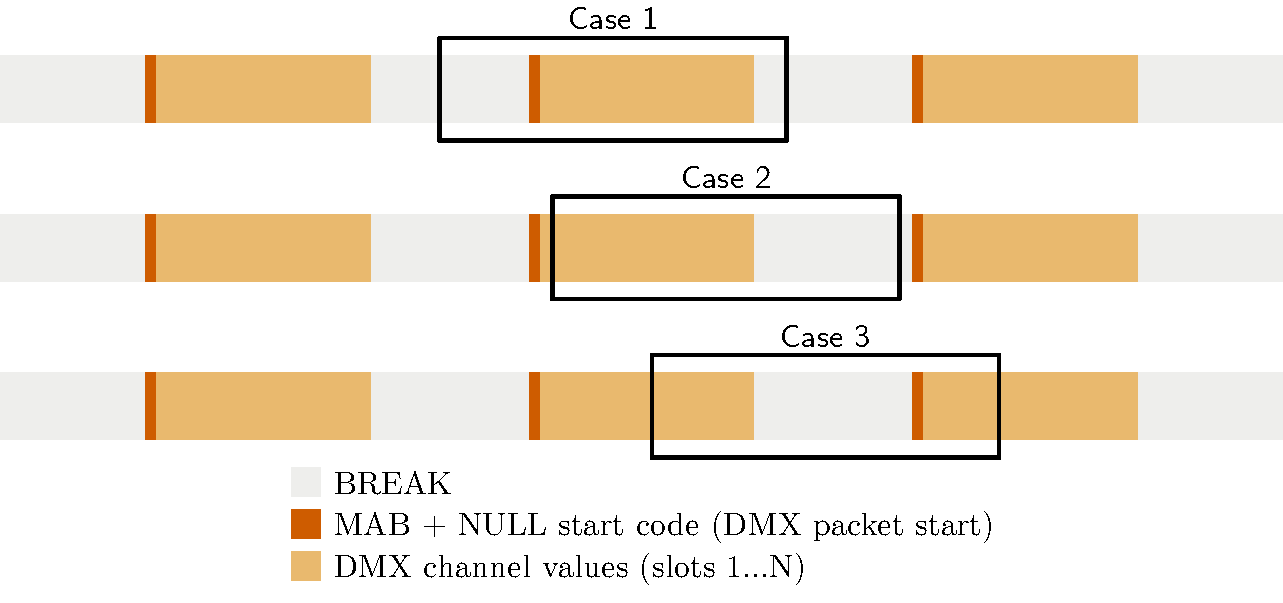
\includegraphics[width=1.00000\textwidth]{Bilder/spi-dmx-chunks.pdf}
\caption[Received SPI chunks versus DMX signal stream]{Received SPI chunks versus DMX signal stream. \emph{(Note:
Sizes and proportions are not to scale.)} DMX packets can be either
fully enclosed in one SPI chunk (case 1; this is the optimum case) or
only partially. If only the end of a DMX packet is contained (case 2),
the chunk is useless. If a DMX packet's start is included (case 1 and
case 3), all channel values until the chunk end can be correlated to
their respective channel numbers. Since it is less likely that a DMX
packet starts right at the chunk's beginning than somewhere in the
middle, higher channels are updated less
often.}\label{fig:spi-dmx-chunks}
\end{figure}

\subsubsection{Parsing received SPI
chunks}\label{parsing-received-spi-chunks}

As mentioned earlier, receiving the raw signal requires implementing
parsing the DMX channel values from the sampled data myself. This
parsing has to obey timing constraints of the
\protect\hyperlink{sec:dmx-protocol}{DMX protocol}.

My approach to implementing this is a state machine that processes the
sampled data bit by bit, proceeds to the next state if the received data
follow the DMX protocol and goes back to the initial state otherwise. A
flow chart of this state machine is pictured in
\cref{fig:spi-dmx-state-machine}.

After a DMX slot's start bit is detected, always the middle of the
following 8 DMX bits (= 8 ``SPI bytes'') is sampled to construct the
channel value. The subsequent stop bits decide how to proceed:

\begin{enumerate}
\def\labelenumi{\alph{enumi})}
\tightlist
\item
  Either the two stop bits are \colorbox{WhiteSmoke}{\lstinline!high!} and arbitrarily many
  \colorbox{WhiteSmoke}{\lstinline!high!} bits as \emph{mark between slots} / \emph{mark before
  BREAK} follow. Then, at the next falling edge, the parser saves the
  constructed DMX channel value to the correct position and continues in
  the \emph{in data start bit} state for the next slot. An exception is
  the last channel: If the just saved DMX value was written to channel
  512, then it is clear that no more slots can follow, so the DMX packet
  is completed and the state gets changed to \emph{in BREAK} instead.
\item
  Or there are \colorbox{WhiteSmoke}{\lstinline!low!} bits where the stop bits should be. If
  the constructed channel value is also zero, that was actually not a
  data slot, but the beginning of the BREAK. So all channel values from
  here on are set to zero, the DMX packet is completed and the state
  machine proceeds to \emph{in BREAK}.
\end{enumerate}

\begin{figure}
\centering
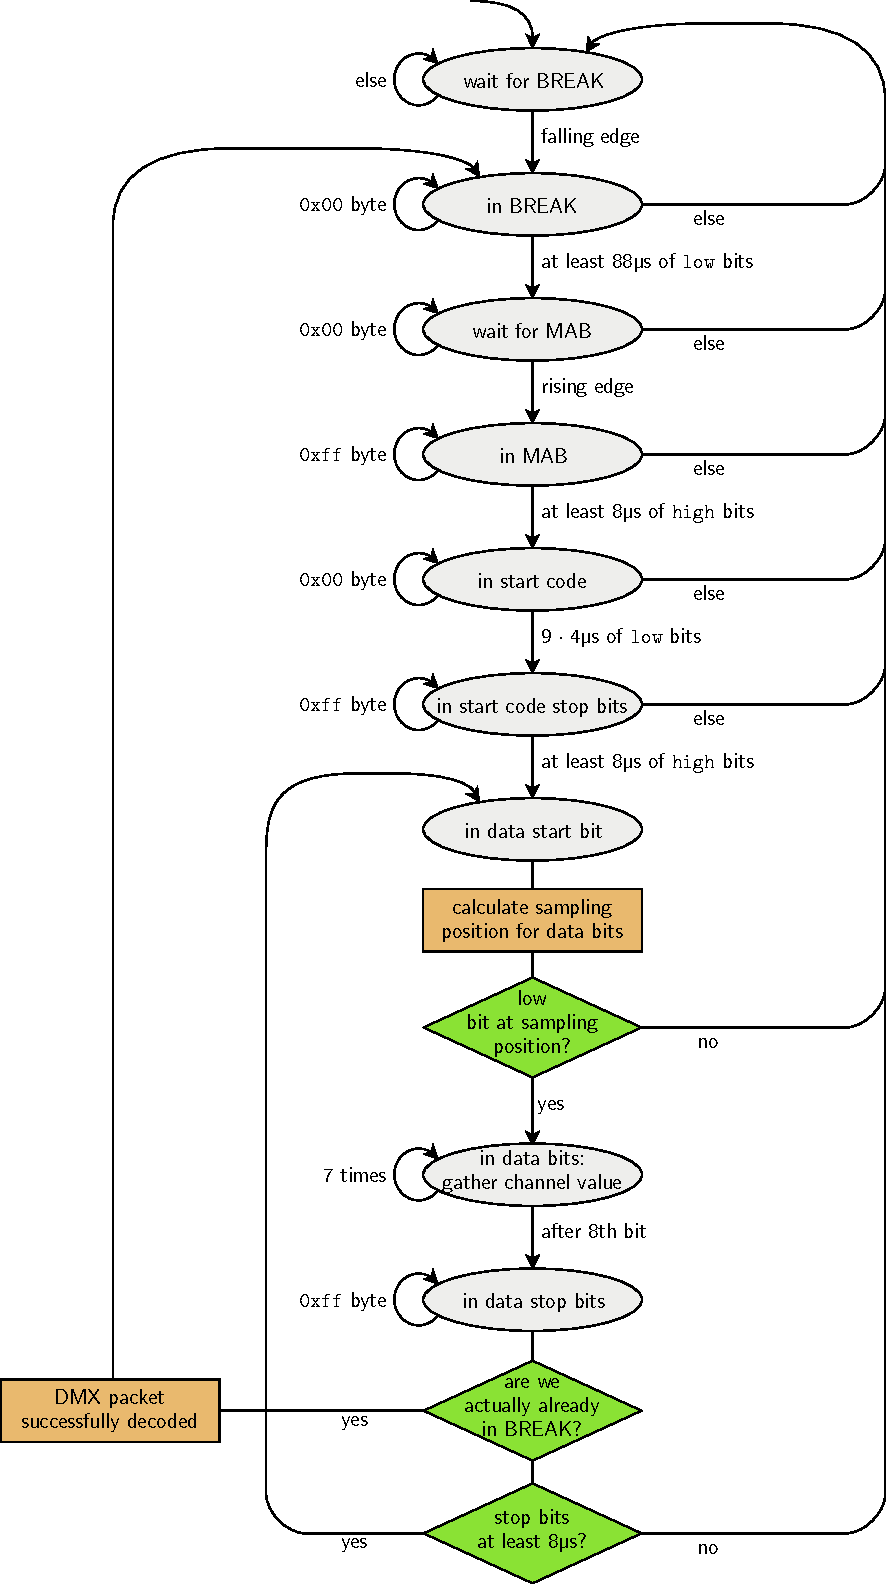
\includegraphics[width=0.79000\textwidth]{Bilder/spi-dmx-state-machine.pdf}
\caption[Parsing DMX from sampled SPI data with a state
machine]{Parsing DMX from sampled SPI data with a state
machine.}\label{fig:spi-dmx-state-machine}
\end{figure}

\glsadd[format=(]{spidmx:SPIDMXParser.cpp}To recognize falling and
rising edges, I wrote two helper functions.
\colorbox{WhiteSmoke}{\lstinline!DetectFallingEdge!} returns the number of zeros if the passed
byte has the form \(1^n 0^{8-n}\) (\(n \in \{ 0, …, 7 \}\)), and -1
otherwise. Note that this case can occur if the byte contains either
only ones or random spikes. \colorbox{WhiteSmoke}{\lstinline!DetectRisingEdge!} works
equivalently.

I show the \colorbox{WhiteSmoke}{\lstinline!WaitForMab!} function as a simple state handler
example. It looks for the first rising edge after the BREAK to change to
the \colorbox{WhiteSmoke}{\lstinline!IN_MAB!} state.

\begin{lstlisting}[numbers=left, style=myCpp, firstnumber=259, caption={[Excerpt from \glsfont{SPIDMXParser.cpp}]Excerpt from \gls{spidmx:SPIDMXParser.cpp}.}]
void SPIDMXParser::WaitForMab() {
  uint8_t byte = chunk[chunk_bitcount];
  if (byte != 0) {
    int8_t ones = DetectRisingEdge(byte);
    if (ones > 0) {
      ChangeState(IN_MAB);
      state_bitcount = ones;
    } else {
      ChangeState(WAIT_FOR_BREAK);
    }
  }
  chunk_bitcount++;
}
\end{lstlisting}

Another notable state handler is \colorbox{WhiteSmoke}{\lstinline!InDataStartbit!} because it
calculates the sampling position of the DMX data bits. This sampling
position should always be in the middle of a byte, and thus depends on
\colorbox{WhiteSmoke}{\lstinline!state_bitcount!}, i.e.~the number of ``SPI bits'' that belong
to the current state, set by the previous state handler (i.e.
\colorbox{WhiteSmoke}{\lstinline!InStartcodeStopbits!} or \colorbox{WhiteSmoke}{\lstinline!InDataStopbits!}).
Possibly, the middle bit was already contained in the last handled byte,
so the current byte is reset to the previous one in this case.
\Cref{tbl:calc-sampling-pos} lists all possible cases.

\begin{lstlisting}[numbers=left, style=myCpp, firstnumber=385]
void SPIDMXParser::InDataStartbit() {
  uint8_t byte = chunk[chunk_bitcount];

  if (state_bitcount >= 4) {
    // look at the last byte again and don't increase chunk_bitcount
    byte = chunk[chunk_bitcount - 1];
    sampling_position = state_bitcount - 4;
  } else {
    // next byte will be handled in next step as usual
    chunk_bitcount++;
    sampling_position = state_bitcount + 8 - 4;
  }

  // start bit must be zero
  if ((byte & (1 << sampling_position))) {
    ChangeState(WAIT_FOR_BREAK);
  } else {
    current_dmx_value = 0x00;
    ChangeState(IN_DATA_BITS);
  }
}
\end{lstlisting}

\hypertarget{tbl:calc-sampling-pos}{}
\begin{longtable}[]{@{}ccccc@{}}
\caption[Calculating the sampling position
in \colorbox{WhiteSmoke}{\lstinline!InDataStartbit!} state handler]{\label{tbl:calc-sampling-pos}Calculating the sampling position
in \colorbox{WhiteSmoke}{\lstinline!InDataStartbit!} state handler. \colorbox{WhiteSmoke}{\lstinline!d!} represents a
data bit. The desired sampling position is indicated with an arrow.
}\tabularnewline
\toprule
\begin{minipage}[b]{0.13\columnwidth}\centering\strut
state bit count\strut
\end{minipage} & \begin{minipage}[b]{0.26\columnwidth}\centering\strut
previous byte,\\
 current byte\strut
\end{minipage} & \begin{minipage}[b]{0.18\columnwidth}\centering\strut
backtrack?\strut
\end{minipage} & \begin{minipage}[b]{0.14\columnwidth}\centering\strut
new current byte\strut
\end{minipage} & \begin{minipage}[b]{0.14\columnwidth}\centering\strut
sampling bit number\strut
\end{minipage}\tabularnewline
\midrule
\endfirsthead
\toprule
\begin{minipage}[b]{0.13\columnwidth}\centering\strut
state bit count\strut
\end{minipage} & \begin{minipage}[b]{0.26\columnwidth}\centering\strut
previous byte,\\
 current byte\strut
\end{minipage} & \begin{minipage}[b]{0.18\columnwidth}\centering\strut
backtrack?\strut
\end{minipage} & \begin{minipage}[b]{0.14\columnwidth}\centering\strut
new current byte\strut
\end{minipage} & \begin{minipage}[b]{0.14\columnwidth}\centering\strut
sampling bit number\strut
\end{minipage}\tabularnewline
\midrule
\endhead
\begin{minipage}[t]{0.13\columnwidth}\centering\strut
8\strut
\end{minipage} & \begin{minipage}[t]{0.26\columnwidth}\centering\strut
\colorbox{WhiteSmoke}{\lstinline!00000000 dddddddd!} \small\verb!   ↑             !\strut
\end{minipage} & \begin{minipage}[t]{0.18\columnwidth}\centering\strut
yes\strut
\end{minipage} & \begin{minipage}[t]{0.14\columnwidth}\centering\strut
\colorbox{WhiteSmoke}{\lstinline!00000000!} \small\verb!   ↑    !\strut
\end{minipage} & \begin{minipage}[t]{0.14\columnwidth}\centering\strut
4\strut
\end{minipage}\tabularnewline
\begin{minipage}[t]{0.13\columnwidth}\centering\strut
7\strut
\end{minipage} & \begin{minipage}[t]{0.26\columnwidth}\centering\strut
\colorbox{WhiteSmoke}{\lstinline!10000000 0ddddddd!} \small\verb!    ↑            !\strut
\end{minipage} & \begin{minipage}[t]{0.18\columnwidth}\centering\strut
yes\strut
\end{minipage} & \begin{minipage}[t]{0.14\columnwidth}\centering\strut
\colorbox{WhiteSmoke}{\lstinline!10000000!} \small\verb!    ↑   !\strut
\end{minipage} & \begin{minipage}[t]{0.14\columnwidth}\centering\strut
3\strut
\end{minipage}\tabularnewline
\begin{minipage}[t]{0.13\columnwidth}\centering\strut
6\strut
\end{minipage} & \begin{minipage}[t]{0.26\columnwidth}\centering\strut
\colorbox{WhiteSmoke}{\lstinline!11000000 00dddddd!} \small\verb!     ↑           !\strut
\end{minipage} & \begin{minipage}[t]{0.18\columnwidth}\centering\strut
yes\strut
\end{minipage} & \begin{minipage}[t]{0.14\columnwidth}\centering\strut
\colorbox{WhiteSmoke}{\lstinline!11000000!} \small\verb!     ↑  !\strut
\end{minipage} & \begin{minipage}[t]{0.14\columnwidth}\centering\strut
2\strut
\end{minipage}\tabularnewline
\begin{minipage}[t]{0.13\columnwidth}\centering\strut
5\strut
\end{minipage} & \begin{minipage}[t]{0.26\columnwidth}\centering\strut
\colorbox{WhiteSmoke}{\lstinline!11100000 000ddddd!} \small\verb!      ↑          !\strut
\end{minipage} & \begin{minipage}[t]{0.18\columnwidth}\centering\strut
yes\strut
\end{minipage} & \begin{minipage}[t]{0.14\columnwidth}\centering\strut
\colorbox{WhiteSmoke}{\lstinline!11100000!} \small\verb!      ↑ !\strut
\end{minipage} & \begin{minipage}[t]{0.14\columnwidth}\centering\strut
1\strut
\end{minipage}\tabularnewline
\begin{minipage}[t]{0.13\columnwidth}\centering\strut
4\strut
\end{minipage} & \begin{minipage}[t]{0.26\columnwidth}\centering\strut
\colorbox{WhiteSmoke}{\lstinline!11110000 0000dddd!} \small\verb!       ↑         !\strut
\end{minipage} & \begin{minipage}[t]{0.18\columnwidth}\centering\strut
yes\strut
\end{minipage} & \begin{minipage}[t]{0.14\columnwidth}\centering\strut
\colorbox{WhiteSmoke}{\lstinline!11110000!} \small\verb!       ↑!\strut
\end{minipage} & \begin{minipage}[t]{0.14\columnwidth}\centering\strut
0\strut
\end{minipage}\tabularnewline
\begin{minipage}[t]{0.13\columnwidth}\centering\strut
3\strut
\end{minipage} & \begin{minipage}[t]{0.26\columnwidth}\centering\strut
\colorbox{WhiteSmoke}{\lstinline!11111000 00000ddd!} \small\verb!         ↑       !\strut
\end{minipage} & \begin{minipage}[t]{0.18\columnwidth}\centering\strut
no\strut
\end{minipage} & \begin{minipage}[t]{0.14\columnwidth}\centering\strut
\colorbox{WhiteSmoke}{\lstinline!00000ddd!} \small\verb!↑       !\strut
\end{minipage} & \begin{minipage}[t]{0.14\columnwidth}\centering\strut
7\strut
\end{minipage}\tabularnewline
\begin{minipage}[t]{0.13\columnwidth}\centering\strut
2\strut
\end{minipage} & \begin{minipage}[t]{0.26\columnwidth}\centering\strut
\colorbox{WhiteSmoke}{\lstinline!11111100 000000dd!} \small\verb!          ↑      !\strut
\end{minipage} & \begin{minipage}[t]{0.18\columnwidth}\centering\strut
no\strut
\end{minipage} & \begin{minipage}[t]{0.14\columnwidth}\centering\strut
\colorbox{WhiteSmoke}{\lstinline!000000dd!} \small\verb! ↑      !\strut
\end{minipage} & \begin{minipage}[t]{0.14\columnwidth}\centering\strut
6\strut
\end{minipage}\tabularnewline
\begin{minipage}[t]{0.13\columnwidth}\centering\strut
1\strut
\end{minipage} & \begin{minipage}[t]{0.26\columnwidth}\centering\strut
\colorbox{WhiteSmoke}{\lstinline!11111110 0000000d!} \small\verb!           ↑     !\strut
\end{minipage} & \begin{minipage}[t]{0.18\columnwidth}\centering\strut
no\strut
\end{minipage} & \begin{minipage}[t]{0.14\columnwidth}\centering\strut
\colorbox{WhiteSmoke}{\lstinline!0000000d!} \small\verb!  ↑     !\strut
\end{minipage} & \begin{minipage}[t]{0.14\columnwidth}\centering\strut
5\strut
\end{minipage}\tabularnewline
\bottomrule
\end{longtable}

All other state handler functions can be inspected in
\gls{spidmx:SPIDMXParser.cpp}.

The \colorbox{WhiteSmoke}{\lstinline!ParseDmx!} method, which is given an SPI chunk to parse,
iterates through the chunk's bytes and calls the respective state
handlers. Whenever a DMX packet end is detected,
\colorbox{WhiteSmoke}{\lstinline!PacketComplete!} is called, which in turn invokes a callback
function if it has been set before via \gls{spidmx:SPIDMXParser.h}'s
\colorbox{WhiteSmoke}{\lstinline!SetCallback!} method.

\emph{Note:} The code listings above are part of the OLA plugin I wrote.
Details are outlined in the next section. Initially, I tested the code
in a standalone version that could process the output of
\gls{spi-receive.c}'s \colorbox{WhiteSmoke}{\lstinline!printCArray!}
function.\glsadd[format=)]{spidmx:SPIDMXParser.cpp}

\subsubsection{Wrapping the code into an OLA
plugin}\label{sec:spidmx-wrapping}

The final step was to create a new OLA plugin that provides an input
port for every SPI port found on the system. This port can then be
patched to an OLA universe which is forwarded via Art-Net to the
lighting software or directly to a DMX output port.

OLA's \emph{OSC (Open Sound Control) Plugin} includes information about
its development process\footnote{\url{https://github.com/OpenLightingProject/ola/blob/master/plugins/osc/README.developer.md}}
which is a good reference for writing a new plugin. As a name, I chose
\emph{Native SPI DMX Plugin}, following \emph{Native UART DMX Plugin}'s
convention. All classes are prefixed with \colorbox{WhiteSmoke}{\lstinline!SPIDMX!}; their
namespace, as well as directory name, is \colorbox{WhiteSmoke}{\lstinline!spidmx!}. I based the
general plugin structure on UART plugin's:

\begin{itemize}
\tightlist
\item
  The \emph{Plugin} class (\gls{spidmx:SPIDMXPlugin.h}) hooks into OLA's
  plugin infrastructure and searches for SPI devices.
\item
  For every found SPI device, a new OLA \emph{Device}
  (\gls{spidmx:SPIDMXDevice.h}) is instantiated, which in turn creates
  one instance of each of the following classes:

  \begin{itemize}
  \tightlist
  \item
    A \emph{Widget} class (\gls{spidmx:SPIDMXWidget.h}) that abstracts
    away the required \emph{spidev} calls.
  \item
    A \emph{Thread} class (\gls{spidmx:SPIDMXThread.h}) that repeatedly
    calls the Widget's \colorbox{WhiteSmoke}{\lstinline!ReadWrite!} method and saves the
    resulting data. The Thread itself instantiates a new \emph{Parser}
    (\gls{spidmx:SPIDMXParser.h}) to decode the raw SPI data.
  \item
    An \emph{InputPort} class (\gls{spidmx:SPIDMXPort.h}) connects the
    Thread to OLA's plugin mechanism by forwarding DMX data and
    notifying the Thread whenever it is patched or unpatched to / from a
    universe.
  \end{itemize}
\item
  A \gls{spidmx:README.md} document describes the plugin.
\end{itemize}

The UML class diagram in \cref{fig:spidmx-class-diagram} clarifies those
relations.

\begin{figure}
\centering
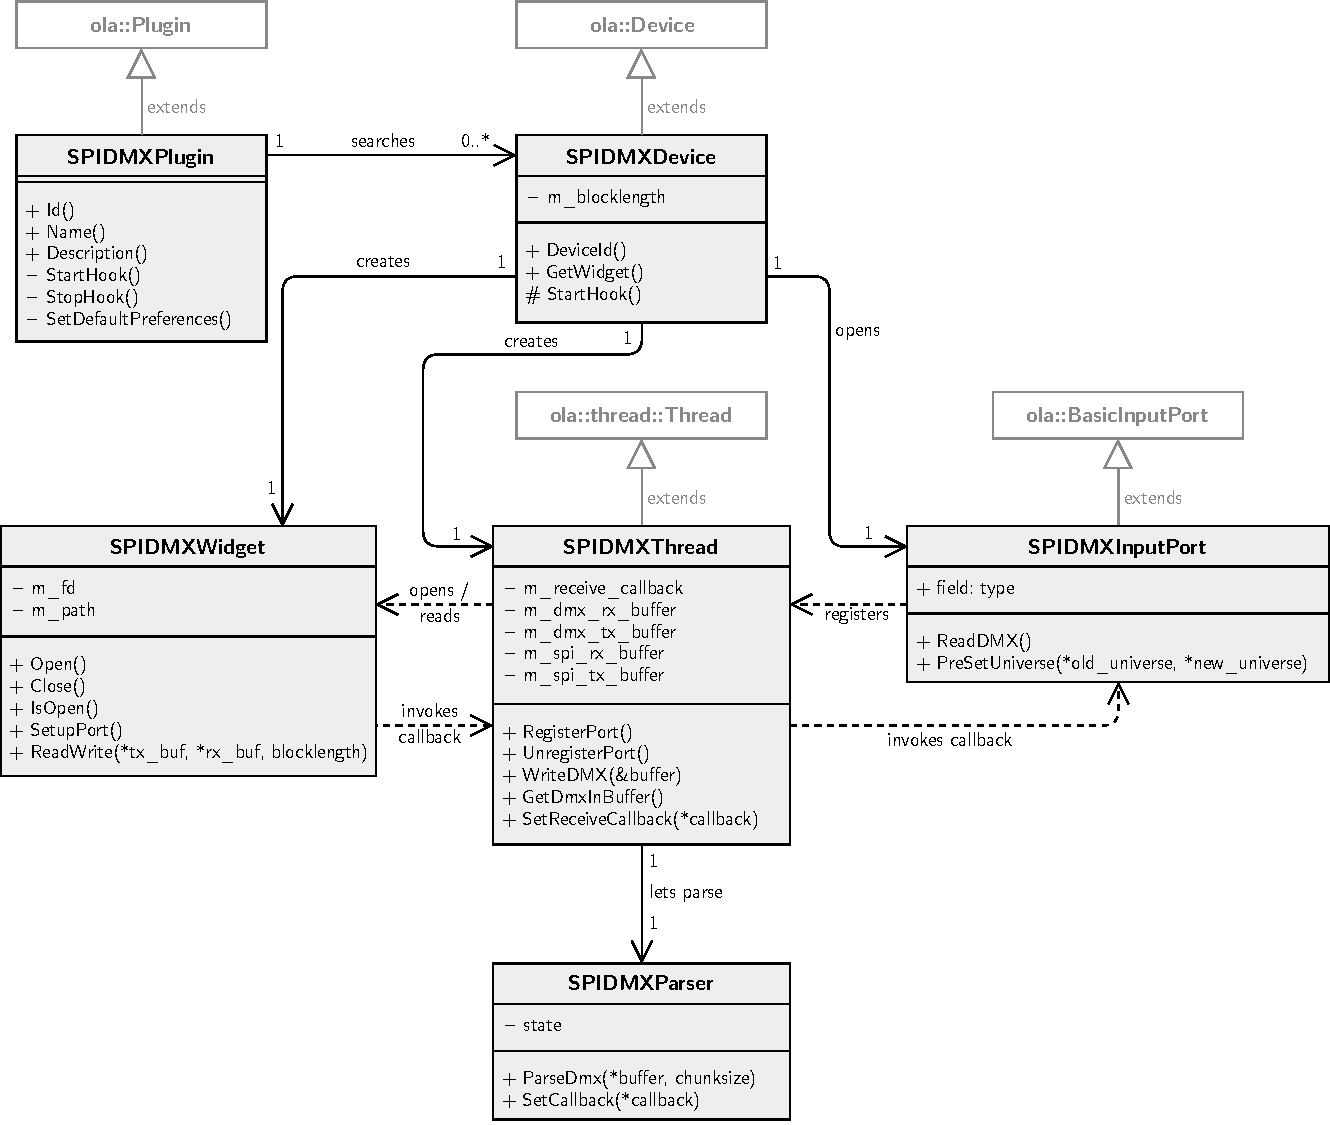
\includegraphics[width=1.00000\textwidth]{Bilder/spidmx-class-diagram.pdf}
\caption[\emph{Native SPI DMX Plugin} UML class diagram]{\emph{Native SPI DMX Plugin} UML class diagram. Note that only
important fields and methods are
included.}\label{fig:spidmx-class-diagram}
\end{figure}

\glsadd[format=(]{spidmx:SPIDMXPort.h}Whenever the Parser detects a DMX
packet end, its \colorbox{WhiteSmoke}{\lstinline!PacketComplete!} function invokes the callback
function that was set in the constructor, called from
\gls{spidmx:SPIDMXThread.cpp}. Its callback in turn is set in
\gls{spidmx:SPIDMXPort.h}'s \colorbox{WhiteSmoke}{\lstinline!PreSetUniverse!} method
(\cref{lst:spidmx-port}) which is always called when the universe that
the port is patched to changes.

This callback chain needs special attention because one has to remember
which pointers could still reference a callback variable, especially as
it could be one in another thread. Mistakes here easily lead to
segmentation faults.

\begin{lstlisting}[numbers=left, style=myCpp, firstnumber=54, caption={[Excerpt from \glsfont{SPIDMXPort.h}]Excerpt from \gls{spidmx:SPIDMXPort.h}.}, label=lst:spidmx-port]
  bool PreSetUniverse(Universe *old_universe, Universe *new_universe) {
    if (!old_universe && new_universe) {
      return m_thread->SetReceiveCallback(NewCallback(
        static_cast<BasicInputPort*>(this),
        &BasicInputPort::DmxChanged));
    }
    if (old_universe && !new_universe) {
      return m_thread->SetReceiveCallback(NULL);
    }
    return true;
  }
\end{lstlisting}

\glsadd[format=)]{spidmx:SPIDMXPort.h}\glsadd[format=(]{configure.ac}Since
plugins can be enabled / disabled at build time, the \emph{autotools}
toolchain must be informed about the new plugin and its operating system
dependencies (namely \emph{spidev}), which was done by adding a single
line to \gls{configure.ac}:

\begin{lstlisting}[numbers=left, firstnumber=836, morekeywords={$have_spi}]
PLUGIN_SUPPORT(spidmx, USE_SPIDMX, [$have_spi])
\end{lstlisting}

\glsadd[format=)]{configure.ac}\glsadd[format=(]{olad:DynamicPluginLoader.cpp}Additionally,
the plugin's \gls{spidmx:Makefile.mk}, which is similar to other
plugins' Makefiles, had to be included from \gls{plugins:Makefile.mk}.

At runtime, the plugin is loaded in \gls{olad:DynamicPluginLoader.cpp},
where the build constant \colorbox{WhiteSmoke}{\lstinline!USE_SPIDMX!} determines if the plugin
was enabled at build time.

\begin{lstlisting}[numbers=left, style=myCpp, firstnumber=215]
#ifdef USE_SPIDMX
  m_plugins.push_back(
      new ola::plugin::spidmx::SPIDMXPlugin(m_plugin_adaptor));
#endif  // USE_SPIDMX
\end{lstlisting}

\glsadd[format=)]{olad:DynamicPluginLoader.cpp}Each plugin is assigned a
plugin ID constant in \gls{Ola.proto}, in this case
\colorbox{WhiteSmoke}{\lstinline!OLA_PLUGIN_SPIDMX = 23!}. It was temporarily 10000 during
development and changed to its final value shortly before merging into
the \colorbox{WhiteSmoke}{\lstinline!master!} branch.

After integrating the new plugin into the existing infrastructure, a
complete rebuild of the project was required:

\begin{lstlisting}[style=myBash]
autoreconf
./configure
make
sudo make install
sudo ldconfig
\end{lstlisting}

The finished SPI DMX Plugin was tested with multiple DMX sources and
works fine. As explained earlier, higher channels are updated less
often, resulting in higher latency. Hence, they should not be used for
light fading, which should be smooth by definition.

The chunk size of one transmission -- which has the largest impact on
this -- is configurable through OLA's plugin settings file
(\colorbox{WhiteSmoke}{\lstinline!/home/pi/.ola/ola-spidmx.conf!}). However, the value of 8192
bytes seems to be a good compromise between a high probability of
including higher channels in a chunk on one hand, and not having too
large uncaptured gaps between chunks on the other.

\emph{Note:} All code changes and additions from this section can be
found in OLA's GitHub pull request 1289\footnote{\url{https://github.com/OpenLightingProject/ola/pull/1289/files}}.

\section{Chassis build}\label{sec:chassis}

To make the DMX interface robust and portable, I housed the Raspberry Pi
together with the \protect\hyperlink{sec:extension-board}{extension
board} in a plastic chassis.

\begin{figure}
\centering
\includegraphics[width=1.00000\textwidth]{Bilder/chassis-parts.png}
\caption[Plastic chassis]{Plastic chassis. Top half with holes for mounting connectors,
bottom half with mounted Raspberry Pi.}
\end{figure}

All external plugs (2 female XLR connectors, 1 male XLR connector, 1
Ethernet jack and 1 power supply plug) are connected via pluggable
extension wires. This allows for a modular installation and easy
replacement of faulty parts. To fit the \emph{DMXCreator 512 Basic} USB
adapter into the chassis, I had to remove its casing, replace its cable
with a more flexible one and enclose it in a heat shrink tube.

\begin{figure}
\centering
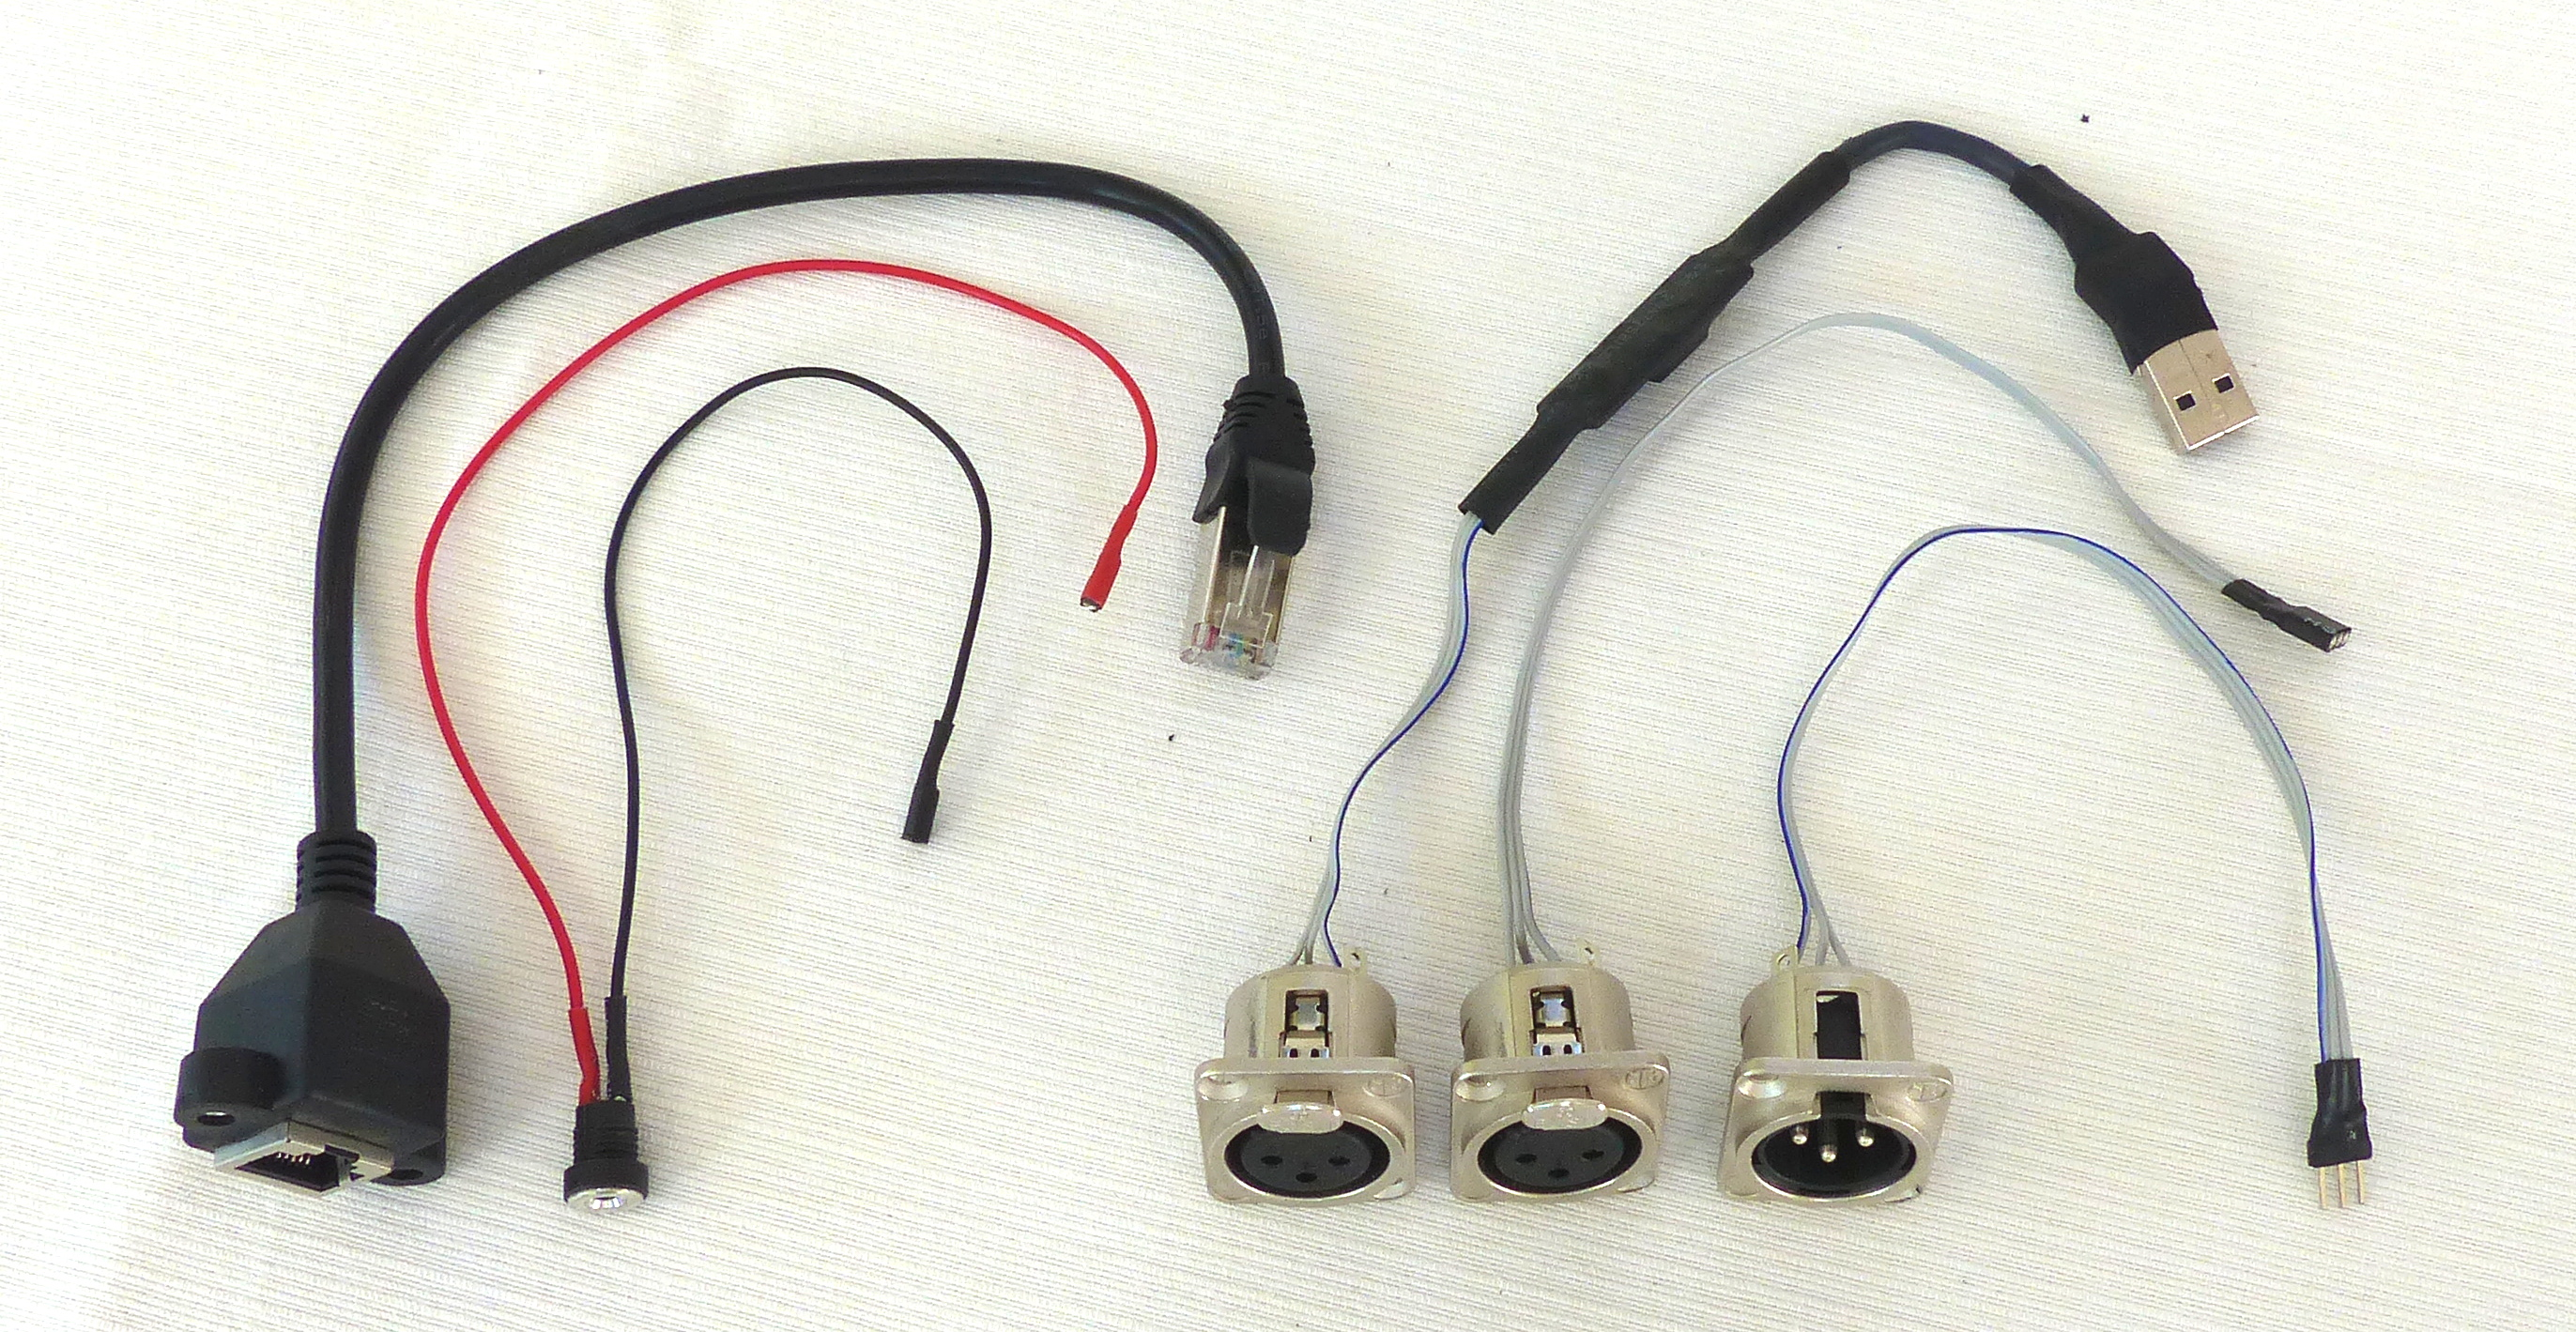
\includegraphics[width=1.00000\textwidth]{Bilder/chassis-cables.jpg}
\caption[Connectors with extension cables]{Connectors with extension cables.}
\end{figure}

Because Raspberry Pi's indicator LEDs are useful to know if it has
powered up and booted correctly, I mounted transparent plastic cords
that act as optical waveguides.

\begin{figure}
\centering
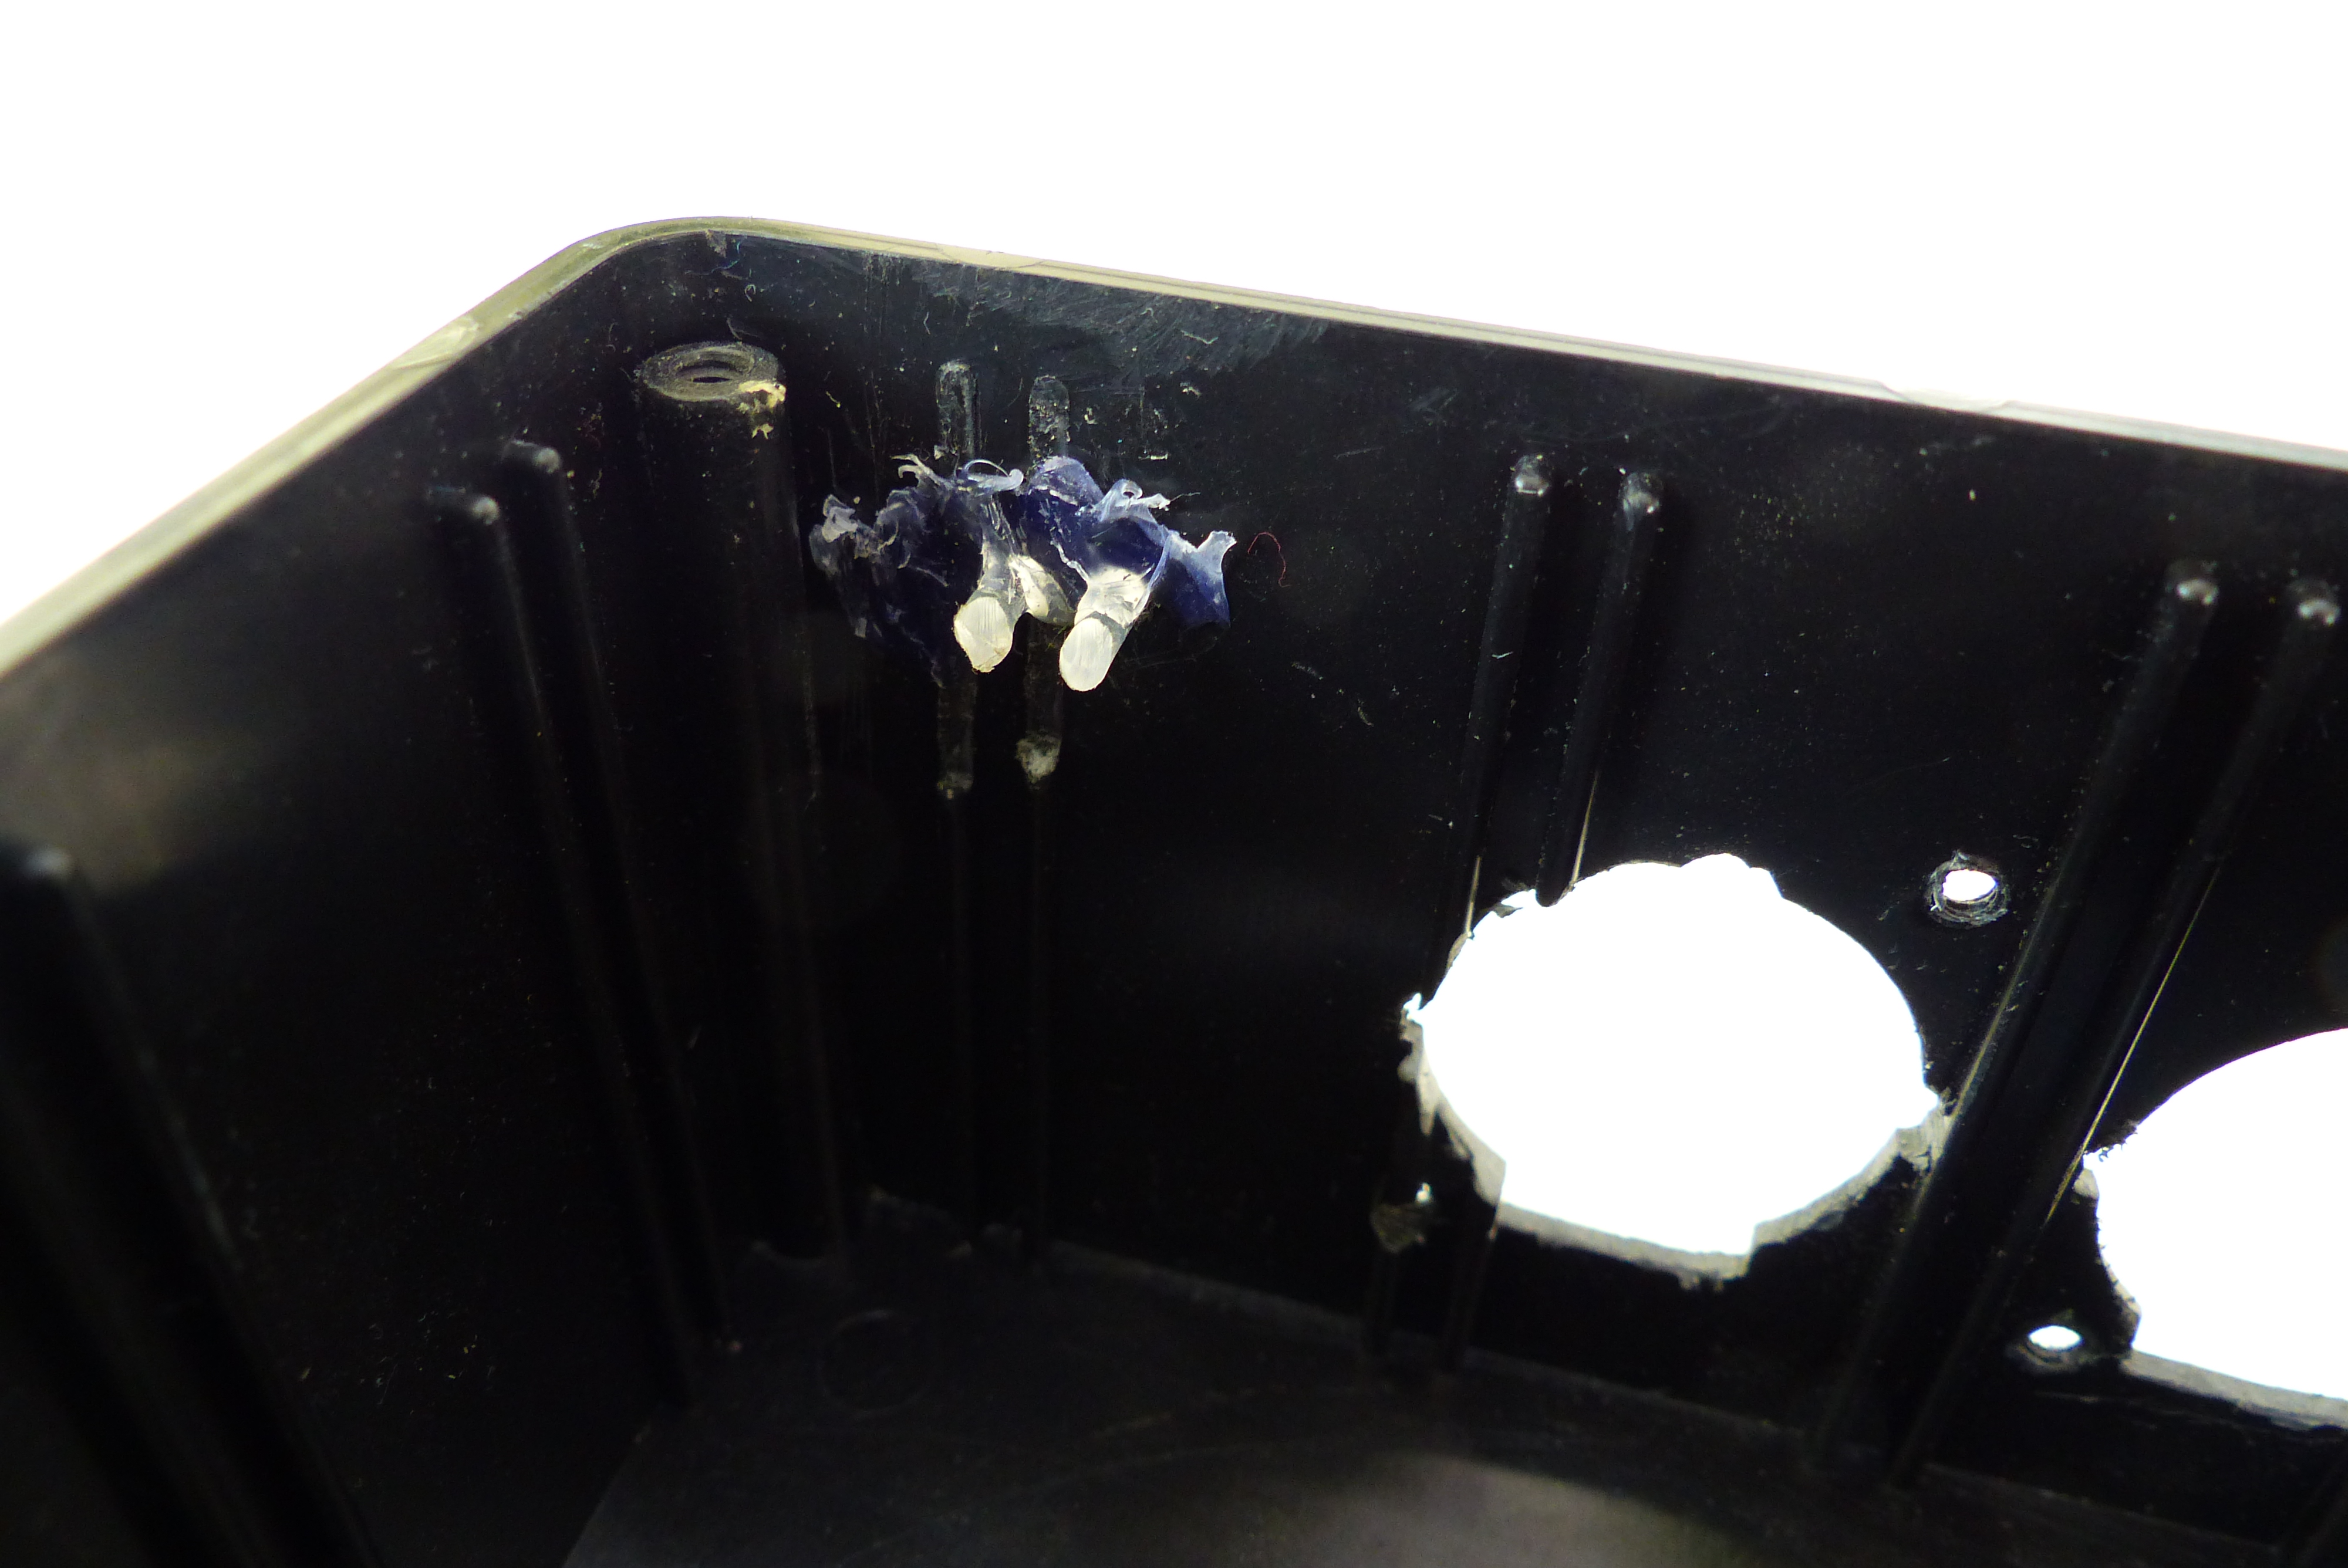
\includegraphics[width=0.75000\textwidth]{Bilder/chassis-indicator-leds.jpg}
\caption[Optical waveguides for indicator LEDs]{Optical waveguides for indicator LEDs.}
\end{figure}

\begin{figure}
\centering
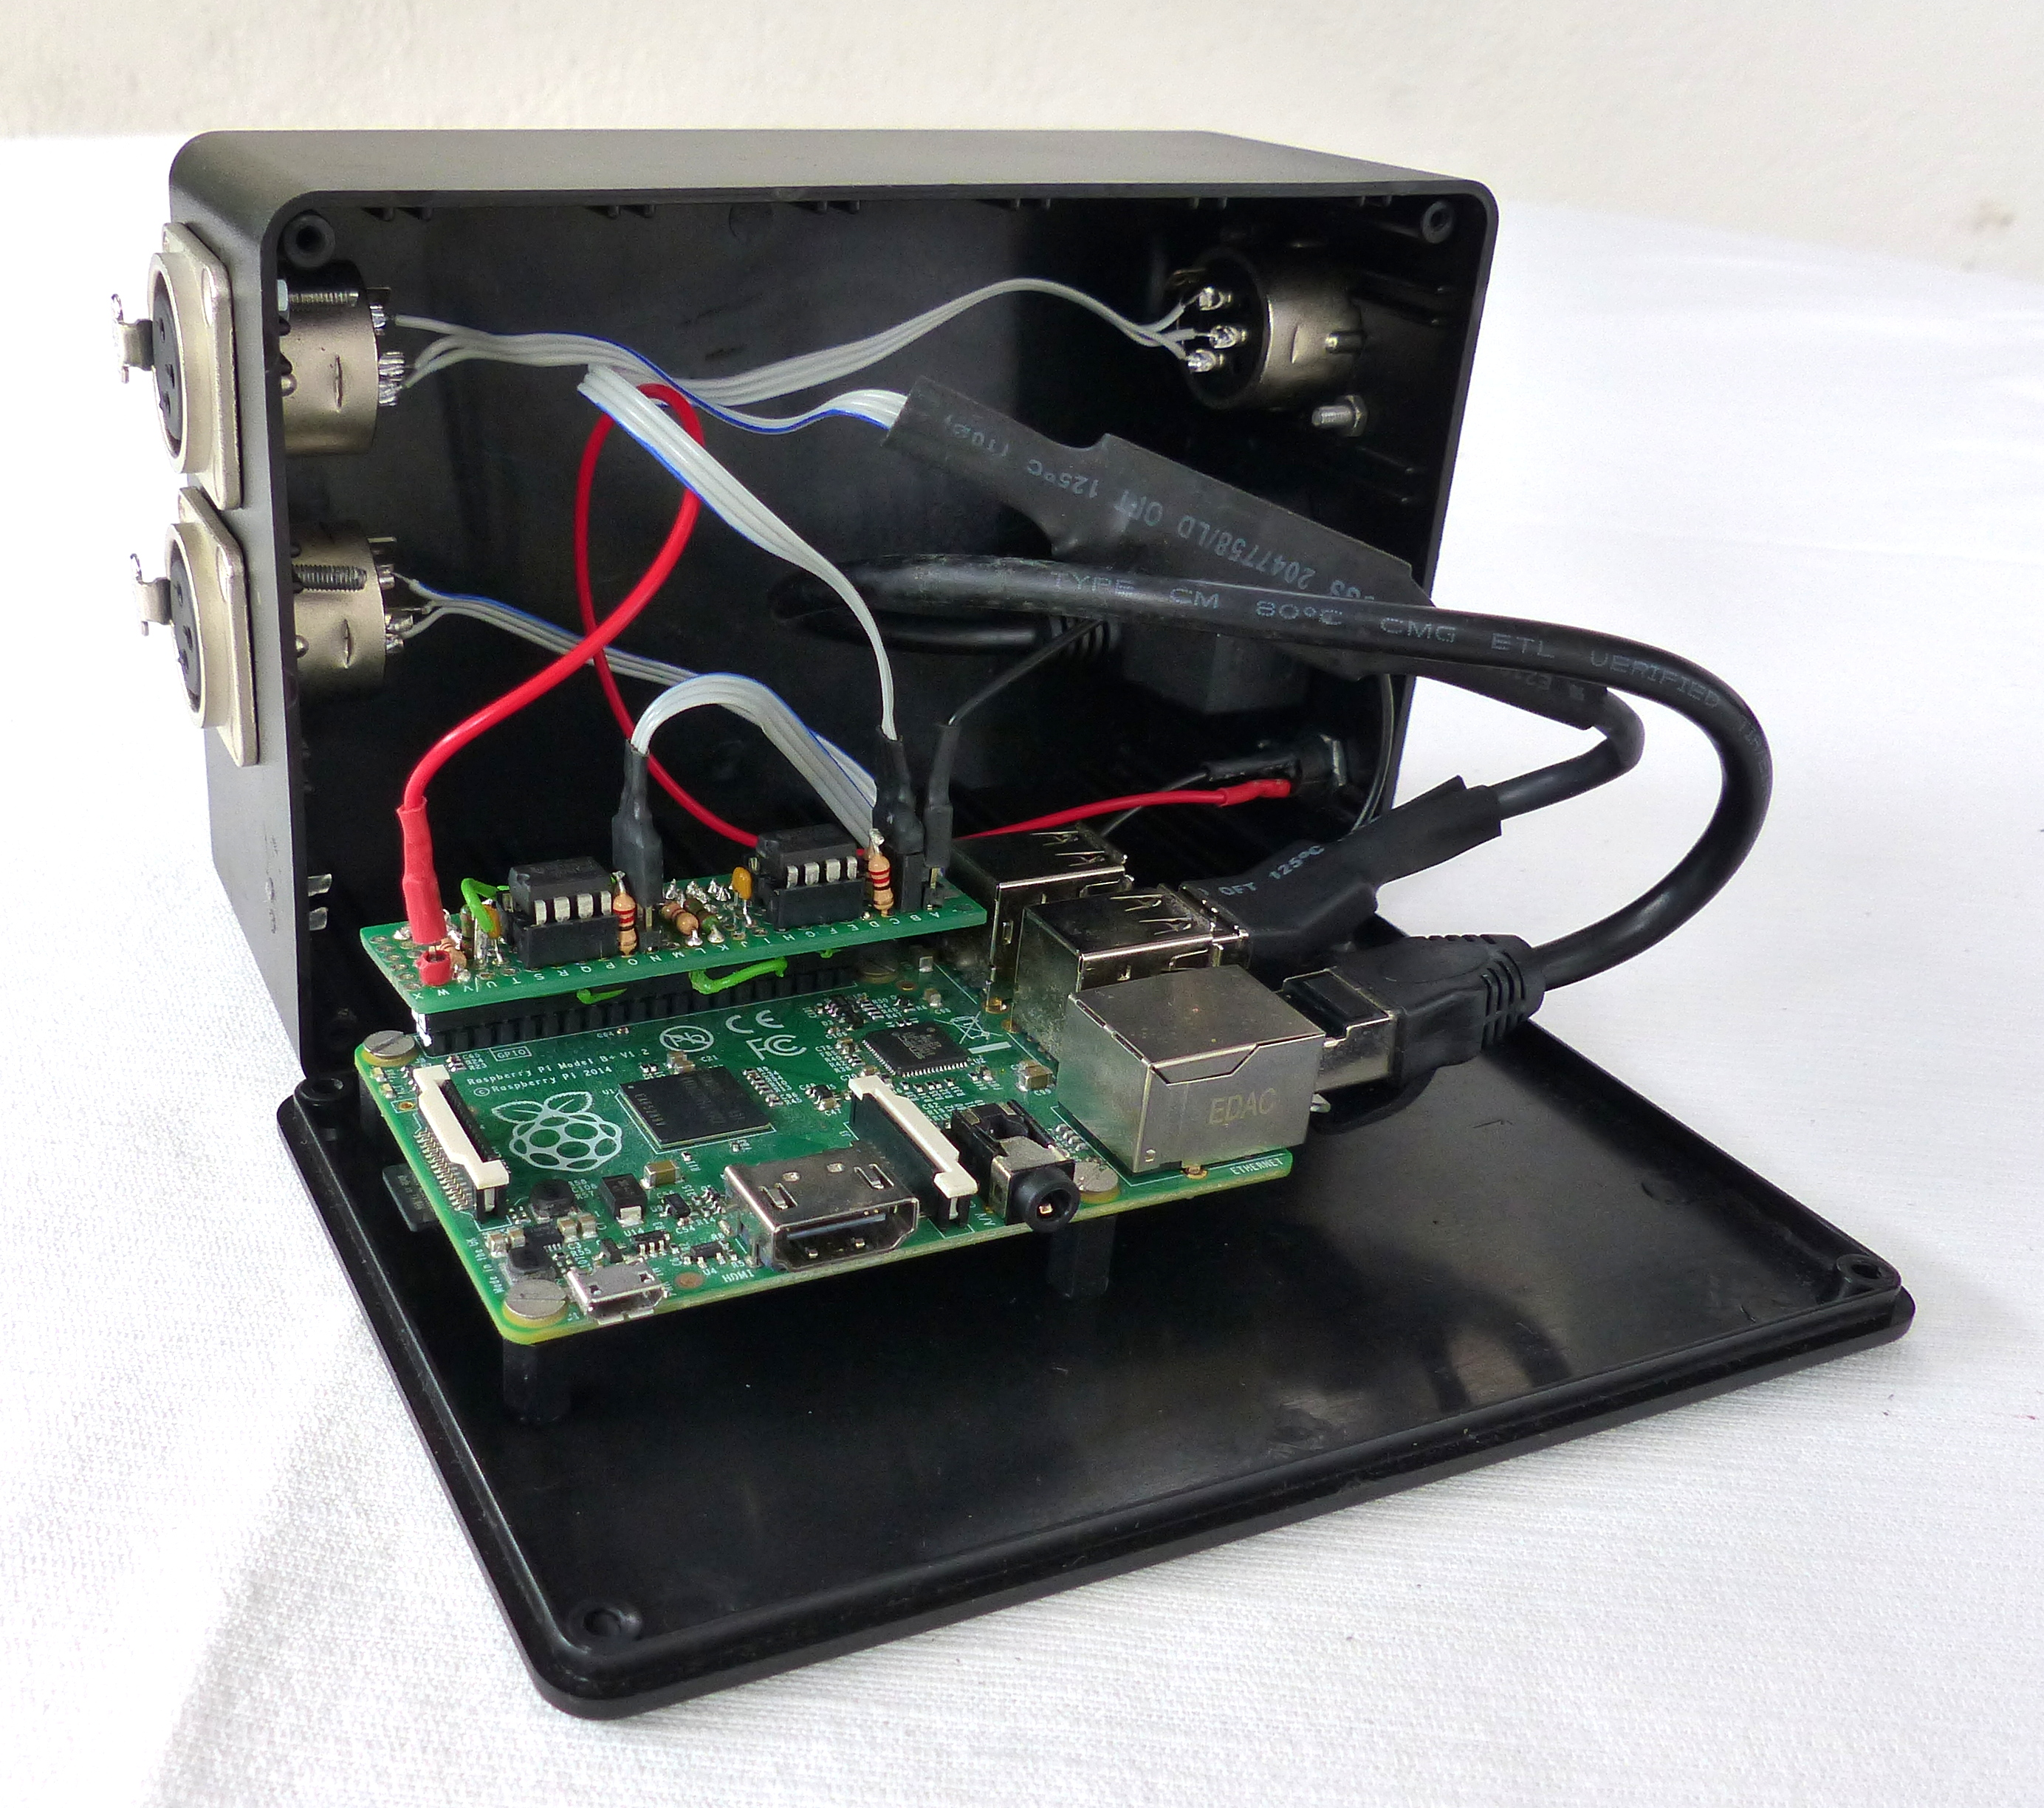
\includegraphics[width=0.75000\textwidth]{Bilder/chassis-open.jpg}
\caption[Open chassis with all connectors mounted and connected]{Open chassis with all connectors mounted and connected.}
\end{figure}

\begin{figure}
\centering
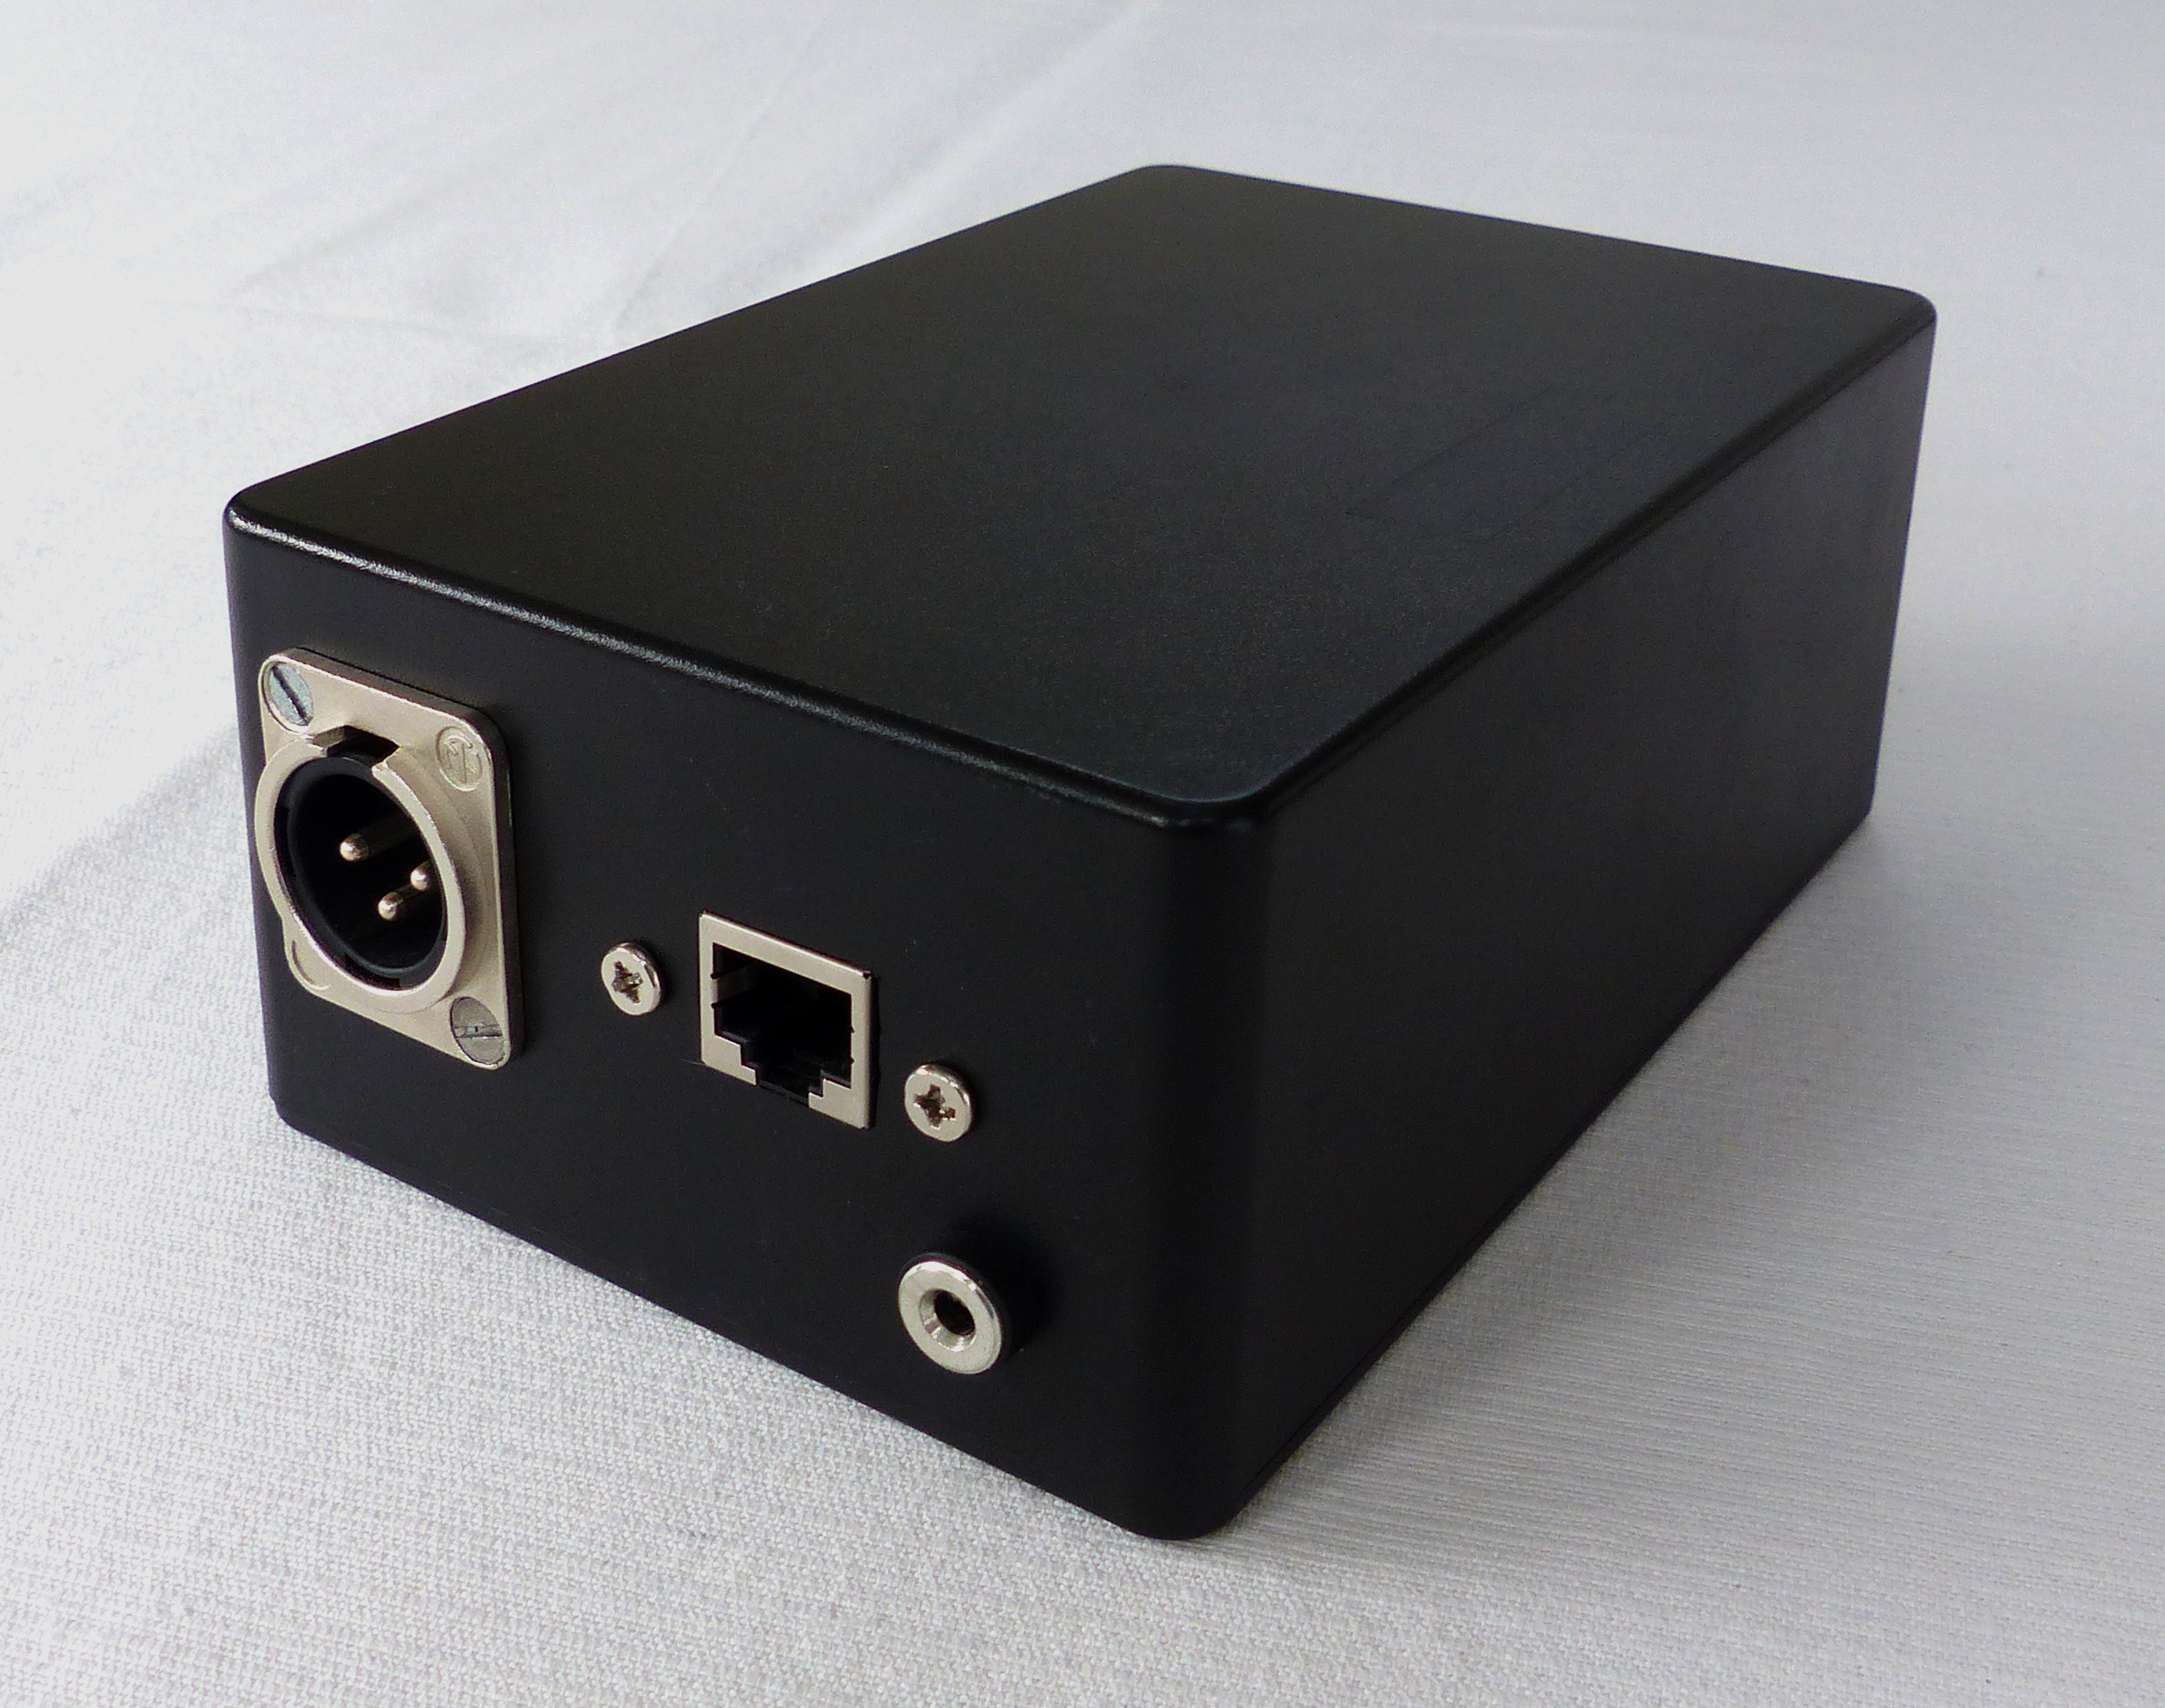
\includegraphics[width=0.75000\textwidth]{Bilder/chassis-finished-front.jpg}
\caption[Finished PC-DMX interface]{Finished PC-DMX interface.}
\end{figure}

\cleardoublepage\hypertarget{sec:testing}{\chapter{Validation}\label{sec:testing}}

The PC-DMX interface
\protect\hyperlink{sec:implementation}{implementation} -- both hardware
and software -- needs to work reliably. This means in particular that it
should fulfill all requirements I defined in \cref{sec:requirements} at
all times, except when outer circumstances, e.g.~power loss, prevent it
from doing so.

Code quality checks and unit tests can help as automatic tools to ensure
this. However, as I will outline in the first subsection, I cannot fully
rely on them.

\section{Unit tests}\label{unit-tests}

The Open Lighting Architecture project provides a test infrastructure
and various existing tests. My code changes and additions did not cause
these existing tests to fail, which suggests that no regressions were
introduced.

Testing the new code with actual hardware support is very difficult. A
DMX signal would have had to be sent through an output port back into an
input port to check its delay and data integrity. That procedure would
depend on two plugins and thereby violate the principle of isolation for
unit tests: If the test fails, it is not clear which of the components
caused it to. Also, hardware testing is not automatable in continuous
integration tools.

Instead, I manually tested the PC-DMX interface's functionality by
connecting light fixtures and comparing expected and observed light
output. Indeed, the interface was already successfully deployed at
several events that lasted for around 10 hours. It ran stable for the
whole period of time, indicating that no mistakes were made in the
implementation that would noticeably affect the behavior.

\section{Code quality}\label{code-quality}

To ensure a high code quality standard, the OLA project has defined a
code style that has to be adhered to. The automatic \emph{lint checks}
that are run after every commit in GitHub pull requests to prevent
violation are fulfilled by my code changes.

The consistent code style improves readability, which makes careful
reviews by the project maintainers in the GitHub pull requests easier.
Discussion there also helped find bugs and inconsistencies before
merging the new features into the \colorbox{WhiteSmoke}{\lstinline!master!} branch.

\section{Fulfillment of
requirements}\label{sec:fulfillment-requirements}

Many of the requirements are already fulfilled by OLA as the software
basis. That applies to supporting different lighting control programs
using both proprietary and open network protocols, ease of use through
the web interface and being open-source. Also, OLA directly allows
flexibly patching DMX inputs and outputs to universes, which permits all
wanted use cases and possibly even more.

Two DMX outputs and one DMX input are supported right now, more can be
added by simply connecting appropriate hardware via USB. DMX output
frequency is satisfactory, which was verified manually by connecting
light fixtures at different DMX addresses and fading them smoothly using
a lighting control software. DMX input is also picked up often enough to
allow smooth fading for approximately the lower 400 channels, fading
higher channels feels rough.

The costs of Raspberry Pi 1 Model B+, 4GB microSD card, circuit board,
electronic components, plug connectors chassis and power supply add up
to about 60\euro{}, staying far below the limit of 100\euro{}. The
\emph{DMXCreator 512 Basic} USB adapter though is not included. It was
apparently sold for over 400\euro{}\footnote{\url{http://vxco.ch/wp-content/uploads/2012/10/DMXCREATOR-_PREISLISTE_CH_D_2.15.pdf}}
before it was discontinued, but it was available to me for free anyway,
so it would not be fair to count it. As substitute, other very cheap
USB-DMX adapters (around 20\euro{}) could possibly be integrated into
OLA with some effort. Other options are mentioned in the next chapter.

\hypertarget{tbl:fulfillment-requirements}{}
{
\renewcommand{\arraystretch}{1.6}
\begin{longtable}[]{@{}ll@{}}
\caption[Fulfillment of requirements]{\label{tbl:fulfillment-requirements}Fulfillment of requirements. See \cref{sec:requirements}.
}\tabularnewline
\toprule
\begin{minipage}[b]{0.54\columnwidth}\raggedright\strut
Requirement\strut
\end{minipage} & \begin{minipage}[b]{0.40\columnwidth}\raggedright\strut
Fulfillment\strut
\end{minipage}\tabularnewline
\midrule
\endfirsthead
\toprule
\begin{minipage}[b]{0.54\columnwidth}\raggedright\strut
Requirement\strut
\end{minipage} & \begin{minipage}[b]{0.40\columnwidth}\raggedright\strut
Fulfillment\strut
\end{minipage}\tabularnewline
\midrule
\endhead
\begin{minipage}[t]{0.54\columnwidth}\raggedright\strut
Works with multiple lighting control programs\strut
\end{minipage} & \begin{minipage}[t]{0.40\columnwidth}\raggedright\strut
\ding{51}\strut
\end{minipage}\tabularnewline
\begin{minipage}[t]{0.54\columnwidth}\raggedright\strut
Connection to computer possible via Ethernet\strut
\end{minipage} & \begin{minipage}[t]{0.40\columnwidth}\raggedright\strut
\ding{51}\strut
\end{minipage}\tabularnewline
\begin{minipage}[t]{0.54\columnwidth}\raggedright\strut
Open protocol between computer and interface supported\strut
\end{minipage} & \begin{minipage}[t]{0.40\columnwidth}\raggedright\strut
\ding{51}\strut
\end{minipage}\tabularnewline
\begin{minipage}[t]{0.54\columnwidth}\raggedright\strut
2 DMX output ports\strut
\end{minipage} & \begin{minipage}[t]{0.40\columnwidth}\raggedright\strut
\ding{51}\strut
\end{minipage}\tabularnewline
\begin{minipage}[t]{0.54\columnwidth}\raggedright\strut
1 DMX input port\strut
\end{minipage} & \begin{minipage}[t]{0.40\columnwidth}\raggedright\strut
\ding{51}\strut
\end{minipage}\tabularnewline
\begin{minipage}[t]{0.54\columnwidth}\raggedright\strut
Input universe handling configurable\strut
\end{minipage} & \begin{minipage}[t]{0.40\columnwidth}\raggedright\strut
\ding{51}\strut
\end{minipage}\tabularnewline
\begin{minipage}[t]{0.54\columnwidth}\raggedright\strut
High refresh rate for DMX input and output\strut
\end{minipage} & \begin{minipage}[t]{0.40\columnwidth}\raggedright\strut
mostly \ding{51}\\
 (higher DMX input channels are refreshed less often, see above)\strut
\end{minipage}\tabularnewline
\begin{minipage}[t]{0.54\columnwidth}\raggedright\strut
Easy usability for end-users\strut
\end{minipage} & \begin{minipage}[t]{0.40\columnwidth}\raggedright\strut
mostly \ding{51}\\
 (computer's network settings have to be changed)\strut
\end{minipage}\tabularnewline
\begin{minipage}[t]{0.54\columnwidth}\raggedright\strut
Costs below 100\euro{}\strut
\end{minipage} & \begin{minipage}[t]{0.40\columnwidth}\raggedright\strut
partially \ding{51}\\
 (\emph{DMXCreator 512 Basic} USB-DMX adapter exceeds limit, see
above)\strut
\end{minipage}\tabularnewline
\begin{minipage}[t]{0.54\columnwidth}\raggedright\strut
Extensible\strut
\end{minipage} & \begin{minipage}[t]{0.40\columnwidth}\raggedright\strut
\ding{51}\strut
\end{minipage}\tabularnewline
\begin{minipage}[t]{0.54\columnwidth}\raggedright\strut
Open-source\strut
\end{minipage} & \begin{minipage}[t]{0.40\columnwidth}\raggedright\strut
\ding{51}\strut
\end{minipage}\tabularnewline
\bottomrule
\end{longtable}}

\cleardoublepage\hypertarget{sec:outlook}{\chapter{Conclusion and future
work}\label{sec:outlook}}

The goal of this thesis was to create an inexpensive yet feature-rich
interface between lighting control software on a computer and DMX
fixtures. The detailed requirements were defined and a market study was
conducted to identify strengths and weaknesses in existing products. No
product fulfilled all requirements, so a system design was developed and
implemented, which included reverse engineering the protocol of a
USB-DMX adapter and sampling the SPI bus.

As a result, the new PC-DMX interface is a big improvement over the
proprietary \emph{e:cue} interface used before in my parish youth:
Haptic input is now possible using any DMX desk console (though not
entirely for a full universe) and it can be used with multiple lighting
control programs to compare their features and concepts.

There are several subjects that can be improved for future versions and
reproductions to make the interface less expensive, more easy to use or
to add extra features.

\paragraph{More Raspberry Pi-native DMX output
ports}\label{more-raspberry-pi-native-dmx-output-ports}

To stay below the limit of 100\euro{} for future replications, the
output port that is currently provided by the \emph{DMXCreator 512
Basic} USB adapter needs to be replaced. If this second output could be
generated directly with Raspberry Pi's hardware, the costs for a USB
adapter would diminish completely.

An approach that looks promising is using the SPI port not only for DMX
input, but also for output, i.e.~making use of the \emph{MOSI} pin as
well. Each DMX channel value would have to be encoded in 11 bytes; one
\colorbox{WhiteSmoke}{\lstinline!low!} byte as the DMX start bit, then one byte for each DMX
data bit and two \colorbox{WhiteSmoke}{\lstinline!high!} bytes as stop bits. In total, this
adds up to 11 · 512 = 5632 bytes, plus some more for the reset sequence,
which is suitable to go together with the current input implementation.

Another idea is bit banging UART output on a GPIO pin. Timing was too
unreliable for parsing DMX input data but things could indeed look
different for output. There is a benchmark measuring GPIO bit banging
speed\footnote{\url{http://codeandlife.com/2012/07/03/benchmarking-raspberry-pi-gpio-speed/}},
which suggests maximum possible speed is not an issue when using a
native C implementation, like \emph{pigpio}'s
\colorbox{WhiteSmoke}{\lstinline!gpioWaveAddSerial!} function\footnote{\url{http://abyz.me.uk/rpi/pigpio/cif.html\#gpioWaveAddSerial}}.
However, inaccurate timing could of course still be a problem, so
further investigation is needed to draw a conclusion.

\paragraph{Remote device management
(RDM)}\label{remote-device-management-rdm}

As explained briefly at the end of \cref{sec:dmx-protocol}, \emph{Remote
Device Management} (\emph{RDM}) is a bidirectional extension to DMX that
allows setting fixture's options remotely. RDM controllers are usually
even more expensive than regular DMX desk consoles and PC interfaces.
OLA has support for RDM internally, but there is currently no way to
receive / transmit RDM packets natively on the Raspberry Pi.

Note that both directions (input / output) need to be supported for RDM.
Thus, the \emph{SPI DMX Plugin} could be modified to support DMX output
(see previous section) and make the input use configurable: Either one
wants to use both input and output ports individually, or only one
output port with RDM support is desired.

\paragraph{Improve network management}\label{improve-network-management}

Another expensive addition to regular DMX systems are so-called
\emph{wireless DMX} solutions, which use radio signals to transmit DMX
data over the air to their respective receivers. Those are useful when a
long distance has to be bridged between the DMX source and the first
lighting fixture.

Since network protocol like Art-Net and sACN can be carried over Wi-Fi
without problems, it would be possible to use it for communication
between the PC-DMX interface and the controlling computer. One would
only need to add a wireless network adapter to both the Raspberry Pi and
the computer (if it is not a laptop with builtin Wi-Fi support anyway)
and connect both to an external access point.

Currently, as one static IP address is set for Raspberry Pi's network
adapter, it is not possible to use multiple PC-DMX interfaces in the
same setup without manually changing the IP addresses to differ from
each other. Additionally, an IP address in the same subnet must be
chosen for the computer, which is tedious extra setup work. Especially
in a wireless system, it would be a desired feature to have them managed
automatically.

An idea would be to have one PC-DMX interface set into \emph{master}
mode, e.g.~with a hardware switch. It then runs a DHCP server and acts
as the access point for all other DMX interfaces in \emph{slave} mode
and also the controlling computer.

\clearpage
\vspace*{2cm}

\begin{center}
    \textbf{Postface}
\end{center}

\vspace*{1cm}

\noindent Since all parts of this PC-DMX interface are open-source,
anybody reading this is welcome to build upon my hardware engineering
and to contribute to the \emph{Open Lighting Architecture} project like
I did. I hope that my work will inspire others to implement their own
PC-DMX interfaces and share their experiences.

For questions and remarks, the author can be contacted via
email\footnote{\href{mailto:florian-edelmann@online.de}{\nolinkurl{florian-edelmann@online.de}}}
or GitHub\footnote{\url{https://github.com/FloEdelmann}}.
